\documentclass[a4paper]{article}
\usepackage{graphicx}
\usepackage{amsmath, amsfonts, geometry, float, listings, enumerate, multicol}
\usepackage{booktabs} 
\usepackage{multicol, float, color, colortbl}
\usepackage{tikz, titlesec, parskip, pgfplots, filecontents}
\usetikzlibrary{shapes,arrows}
\usepackage{enumitem}
\usepackage{amssymb}
\usepackage{hyperref}
\usepackage{mathtools}
\usepackage{braket}
\usepackage{pgfplots}

%\usepackage{listings}
%\usepackage{color}

% Define MATLAB code formatting
\lstdefinestyle{mystyle}{
	language=Matlab,
	backgroundcolor=\color{white},
	commentstyle=\color{green},
	keywordstyle=\color{blue},
	numberstyle=\tiny\color{gray},
	stringstyle=\color{magenta},
	basicstyle=\footnotesize,
	breakatwhitespace=false,         
	breaklines=true,                 
	captionpos=b,                    
	keepspaces=true,                 
	numbers=left,                    
	numbersep=5pt,                  
	showspaces=false,                
	showstringspaces=false,
	showtabs=false,                  
	tabsize=2
} 

\lstset{style=mystyle}

\pgfplotsset{compat = newest}

\titlespacing{\section}{0pt}{10pt}{0pt}
\titlespacing{\subsection}{0pt}{10pt}{0pt}
\titlespacing{\subsubsection}{0pt}{10pt}{0pt}

\usetikzlibrary{calc,patterns,through}
\newcommand{\arcangle}{%
	\mathord{<\mspace{-9mu}\mathrel{)}\mspace{2mu}}%
}

\renewcommand{\baselinestretch}{1.4}
\geometry{
	a4paper,
	total={170mm,257mm},
	left=20mm,
	top=20mm,
}
\usepackage{fancyhdr}
\pagestyle{fancy}
\fancyhf{}
\rhead{\textbf{سیستم های مخابراتی}}
\lhead{\textbf{پروژه }}
\cfoot{(\space \space \space \space \textbf{\thepage}  \space \space \space)}
\renewcommand{\headrulewidth}{1pt}
\renewcommand{\footrulewidth}{1pt}


\usepackage{xepersian}
\setlatintextfont{CMU Serif}
\settextfont{XB Niloofar}
%\setdigitfont{XB Niloofar}
\DefaultMathsDigits

\makeatletter
\bidi@patchcmd{\@Abjad}{آ}{الف}
{\typeout{Succeeded in changing آ into الف}}
{\typeout{Failed in changing آ into الف}}
\makeatother
\PersianAlphs

\begin{document}
	
	\newcommand{\Int}{\int\limits}
	\begin{minipage}{0.6\textwidth}
		\begin{bf}
			\begin{center}
				باسمه تعالی\\
				\vspace{0.25cm}
				دانشگاه صنعتی شریف\\
				\vspace{0.25cm}
				دانشکده مهندسی برق\\
				\vspace{0.5cm}
				
				\large
				سیستم های مخابراتی - گروه دکتر پاکروان \\
				نیم‌سال اول
				03-1402\\
				\Large
				پروژه درس سیتم های مخابراتی\\
				نام و نام خانوادگی :علی یداللهی
				\\
				شماره دانشجویی: 400102233
			\end{center}
		\end{bf}
		\normalsize
	\end{minipage} \hfill
	\begin{minipage}{0.35\textwidth}
		
		\begin{flushleft}
			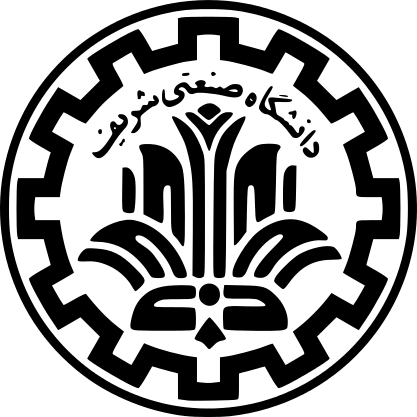
\includegraphics[width=0.6\textwidth]{Shariflogo.png}\\ \large
		\end{flushleft}
		
	\end{minipage}
	
	
	\rule{\textwidth}{1.5pt}
	\large
	\section{مقدمه}
	در این پروژه قصد داریم یک سیستم مخابرات دیجیتال را به طور کامل شبیه سازی کنیم و تأثیر پارامترهای مختلف را بر عملکرد این سیستم مشاهده کنیم. دیاگرام بلوکی فرستنده و گیرنده در شکل های \ref{fig1} و \ref{fig2} نمایش داده شده اند.
		\begin{figure}[h!]
		
		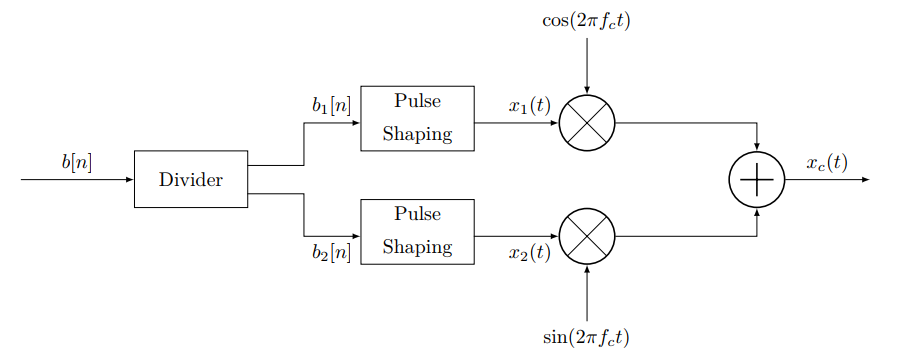
\includegraphics[width=0.8\textwidth]{comsys_fig01.png}\\ 
		\centering
		\caption{دیاگرام بلوکی فرستنده}
		\label{fig1}
	\end{figure}
	\begin{figure}[h!]
		
		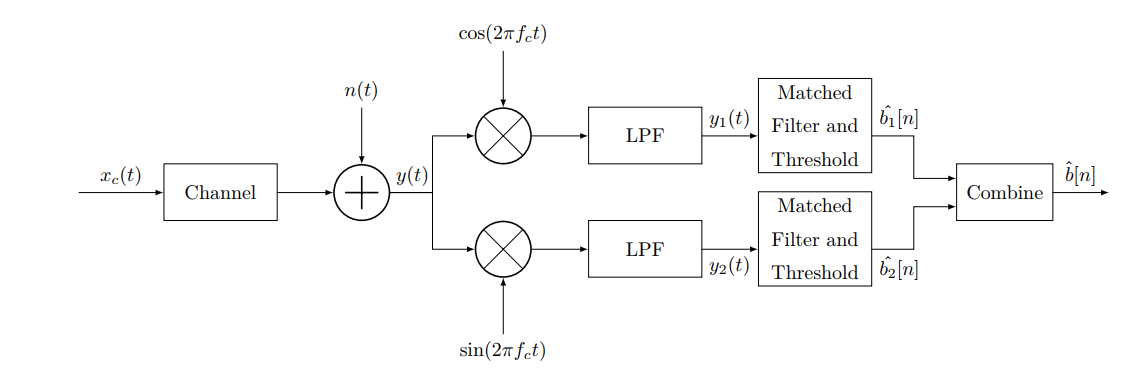
\includegraphics[width=0.8\textwidth]{comsys_fig02.png}\\ 
		\centering
		\caption{دیاگرام بلوکی گیرنده}
		\label{fig2}
	\end{figure}
	\section{پیاده سازی بلوک ها به صورت مجزا}
	\subsection{}
	برای اینکه سیستم به یک سیتم \lr{real-time} نزدیک شود؛هر یک از بیت ها را به صورت یکی درمیان به یکی از دنباله های خروجی می دهیم.
	\subsection{}
	بنابر توضیحات هر وقت در ورودی یک داشتیم شکل پالس یک و هر وقت صفر داشتیم شکل پالس صفر را قرار می دهیم
	\subsection{}
	سیگنال \lr{modulate} را به صورت زیر تولید می کنیم:
	\begin{equation*}
		x_1(t) \cos(2 \pi f_c t) + x_2(t) \sin(2 \pi f_c t)
	\end{equation*} 
	\subsection{}
	از تابع \lr{bandpass} متلب در این قسمت استفاده شده است.
	\subsection{}
	سیگنال خروجی کانال (که ممکن است نویز هم به آن اضافه شده باشد) را یک بار در 
	$\cos (2 \pi f_c t)$
	و یک بار در 
	$\sin (2 \pi f_c t)$
	 ضرب می کنیم و سپس از یک فیلتر \lr{lowpass} با پهنای باند کانال عبور داده و سیگنال های 
	 $y_1(t)$
	 و 
	 $y_2(t)$
	 را تولید می کنیم.
	 \subsection{}
	 از آنجا که \lr{Matched Filter} در واقع کانولوشن سیگنال ورودی با پالس های متناظر با صفر و یک است ؛ روش تصمیم گیری را بر اساس مقدار کانولوشن در لحظات 
	 $nT_b$
	 قرار می دهیم. به طوری که هر کجا سیگنال ورودی مقدار کانولوشن بیشتری با یکی از پالس های صفر یا یک داشت می توانیم تشخیص دهیم که در آن لحظه کدام بیت فرستاده شده است.
\section{انتقال دنباله تصادفی صفر و یک}
\subsection{مولاسیون \lr{PAM}}
\subsubsection*{الف}
دنباله رندوم تولید شده به صورت زیر است:
\begin{figure}[h!]
	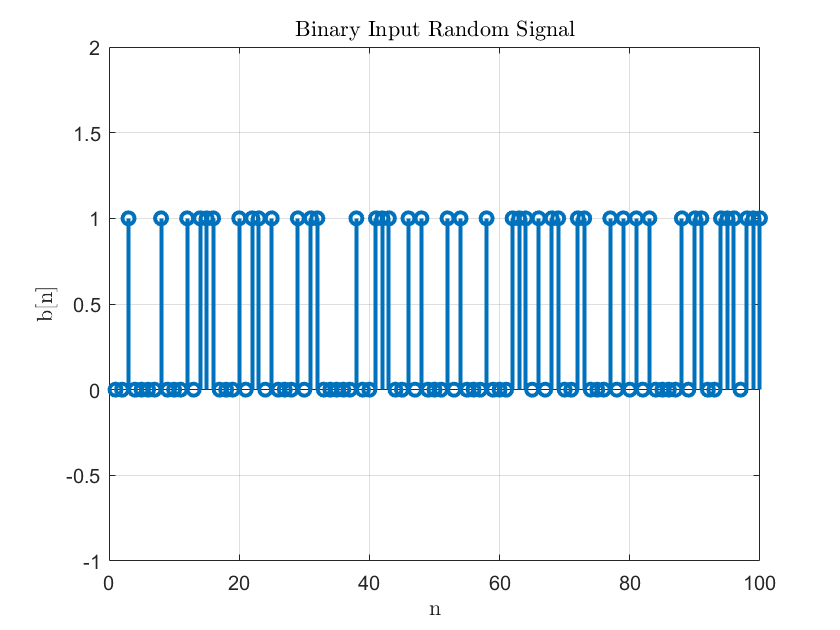
\includegraphics[width=0.5\textwidth]{comsys_fig03.png}\\ 
	\centering
\end{figure}
\newline
پس از عبور از \lr{Devider} دو سیگنال 
$b_1[n]$
و
$b_2[n]$
به دست می آیند.
\newline
\begin{figure}[h!]
	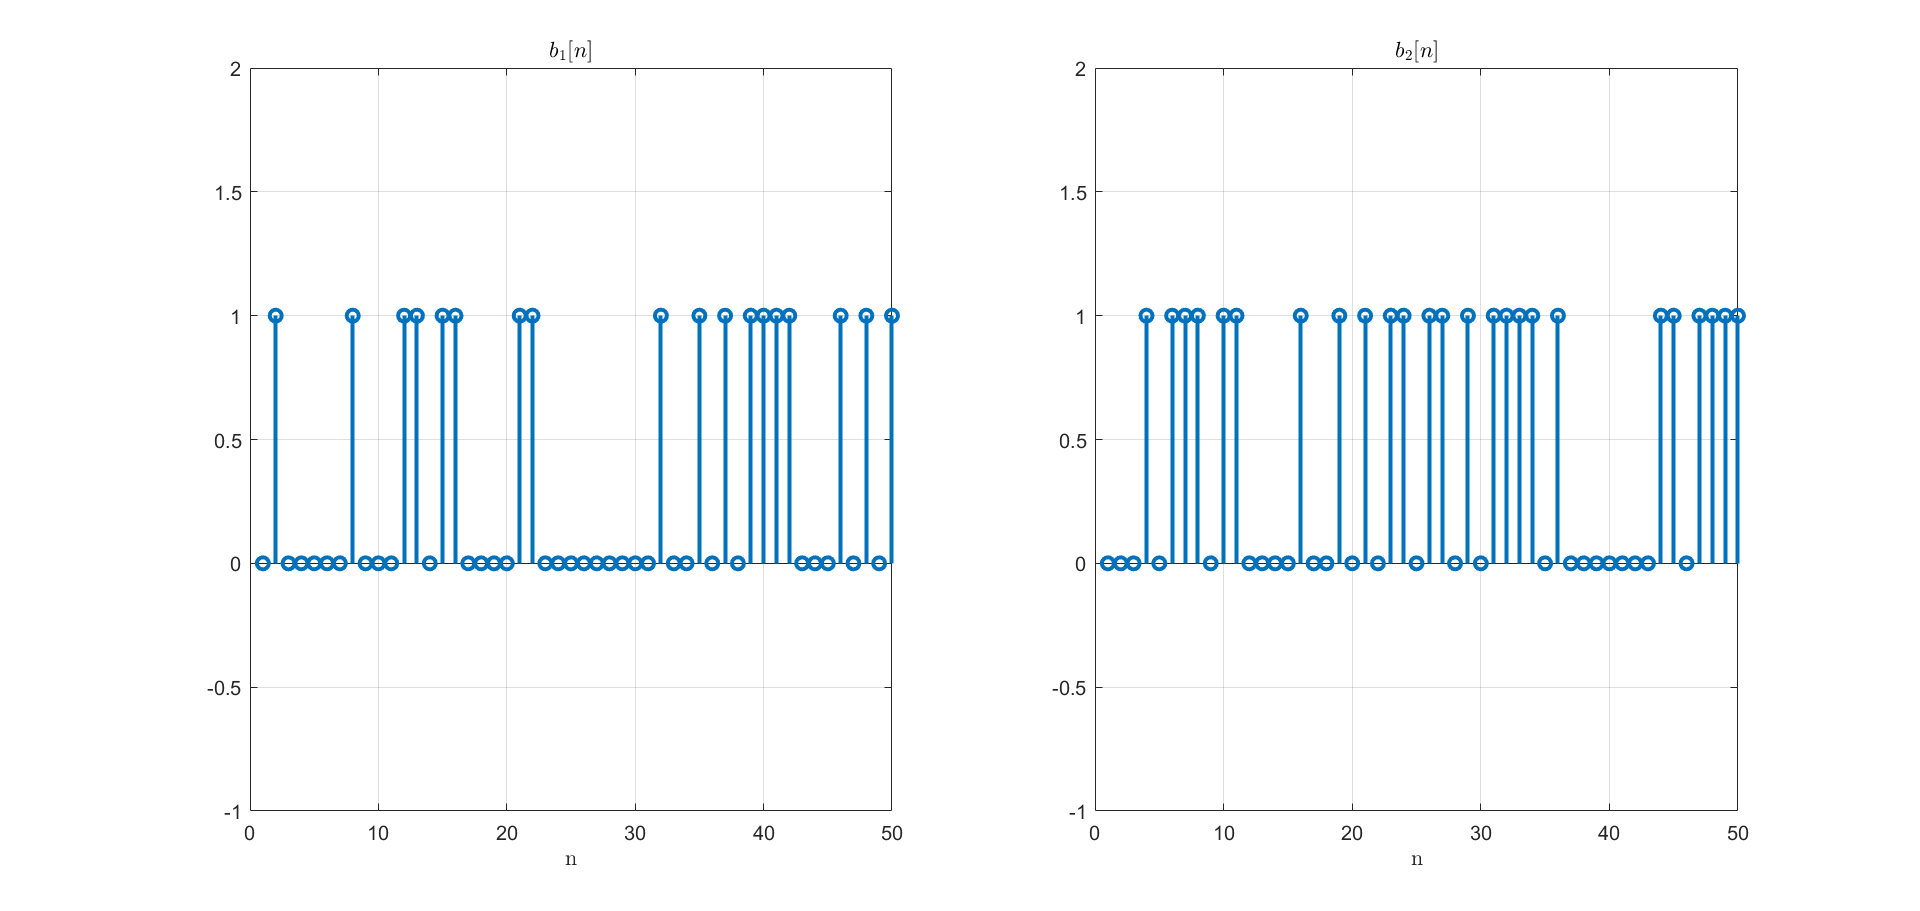
\includegraphics[width=0.8\textwidth]{comsys_fig04.png}\\ 
	\centering
\end{figure}
\newline
بعد از عبور از \lr{Pulse Shaping} سیگنال های 
$x_1(t)$
و 
$x_2(t)$
به دست می آیند.
\newline
\begin{figure}[h!]
	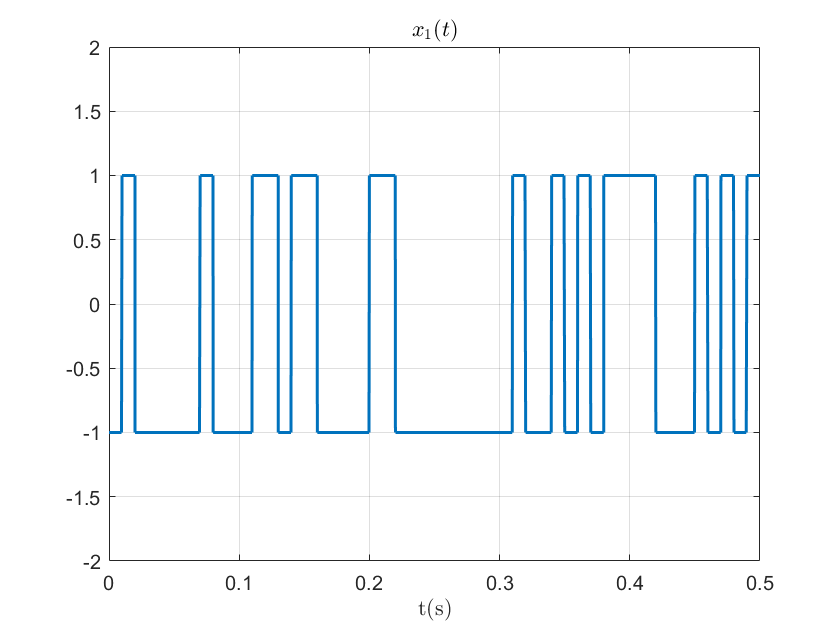
\includegraphics[width=0.5\textwidth]{comsys_fig05.png}\\ 
	\centering
\end{figure}
\begin{figure}[h!]
	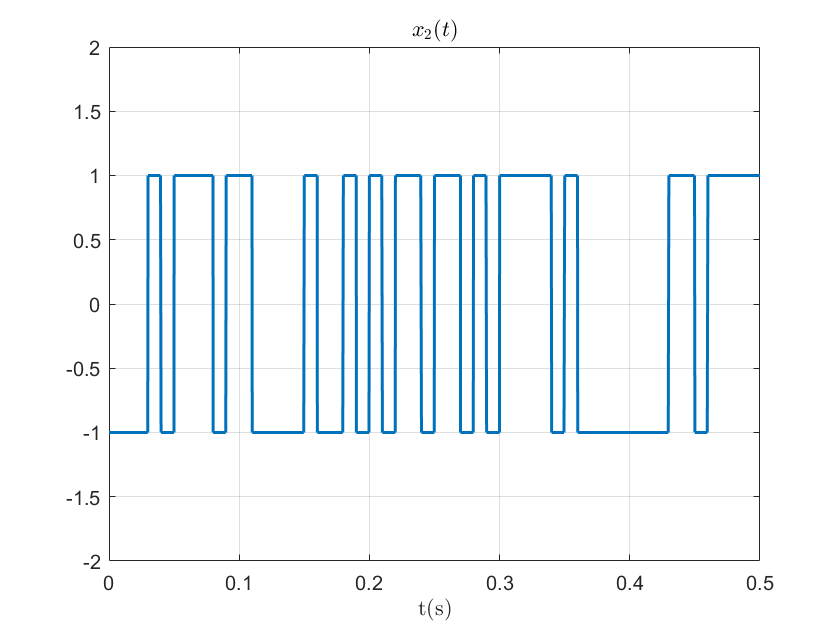
\includegraphics[width=0.5\textwidth]{comsys_fig06.png}\\ 
	\centering
\end{figure}
\newline
پس از عبور از \lr{AnalogMod} ، 
$x_c(t)$
به دست می آید
\newline
\begin{figure}[h!]
	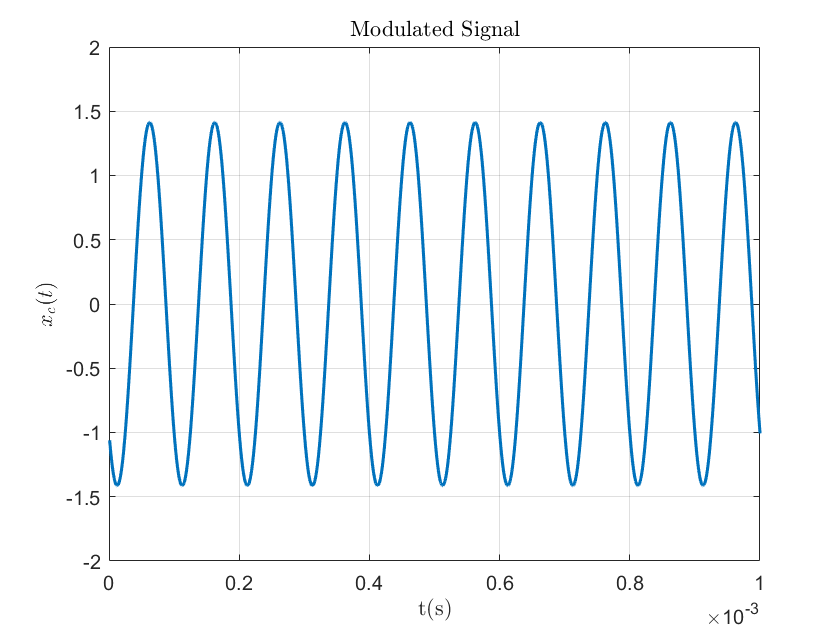
\includegraphics[width=0.7\textwidth]{comsys_fig07.png}\\ 
	\centering
\end{figure}
\newline
	بعد از عبور از کانال به سیگنال 
	$y(t)$
	خواهیم رسید.
	\newline
	\begin{figure}[h!]
		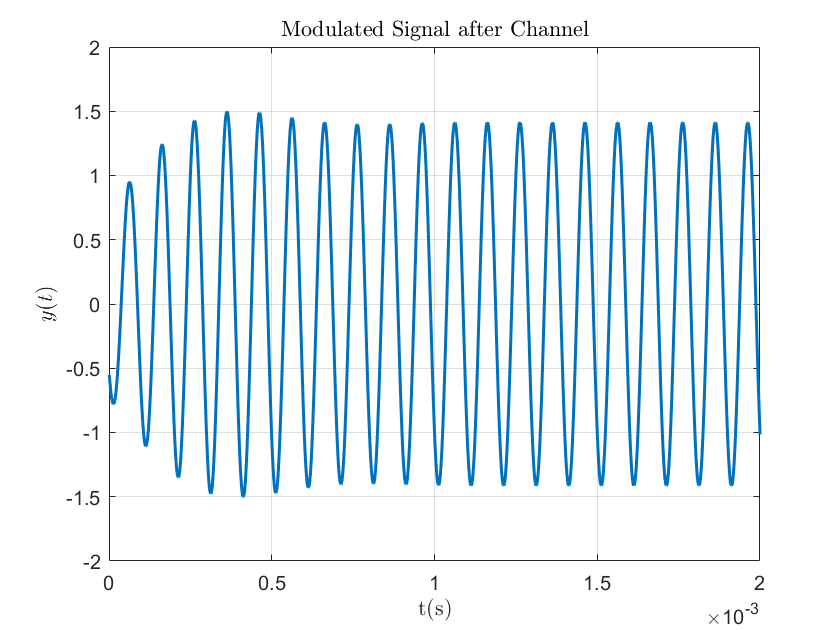
\includegraphics[width=0.7\textwidth]{comsys_fig08.png}\\ 
		\centering
	\end{figure}
	\newpage
	پس از عبور از \lr{AnalogDemod} سیگنال های 
	$y_1(t)$
	و 
	$y_2(t)$
	به دست می آیند.
	\newline
	\begin{figure}[h!]
		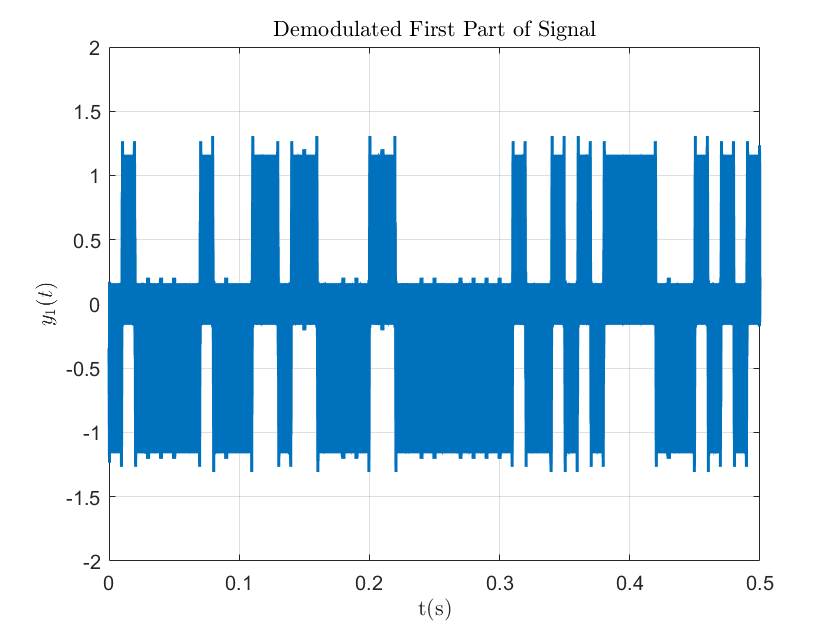
\includegraphics[width=0.45\textwidth]{comsys_fig09.png}\\ 
		\centering
	\end{figure}
	\begin{figure}[h!]
		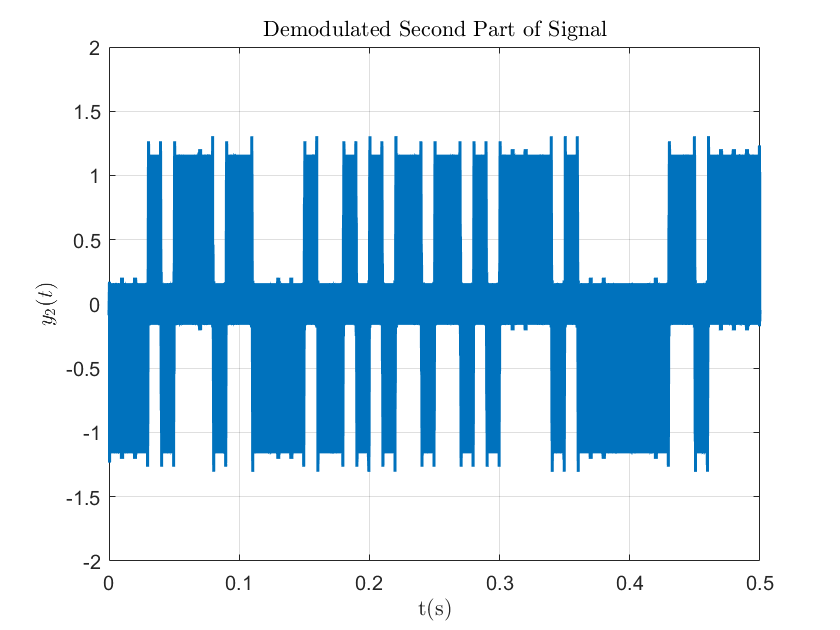
\includegraphics[width=0.45\textwidth]{comsys_fig10.png}\\ 
		\centering
	\end{figure}
	\newline
	حال با استفاده از \lr{Matched Filter} کورولیشن سیگنال ها را با پالس های صفر و یک به دست آورده و به سیگنال های 
	$\hat{b_1}[n]$
	و 
	$\hat{b_2}[n]$
	خواهیم رسید.
	\newline
	مشاهده می شود که هر کجا مقدار کورولیشن با پالس صفر (میله های آبی رنگ) بیشتر بوده مقدار صفر تخمین زده شده و همینطور برای پالس یک
	\newline
	\begin{figure}[h!]
		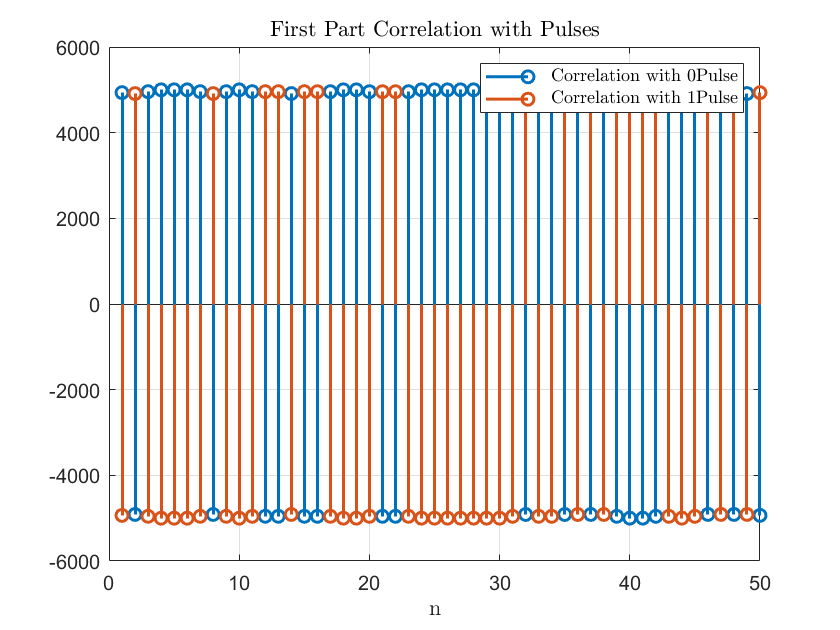
\includegraphics[width=0.4\textwidth]{comsys_fig11.png}\\ 
		\centering
	\end{figure}
	\begin{figure}[h!]
		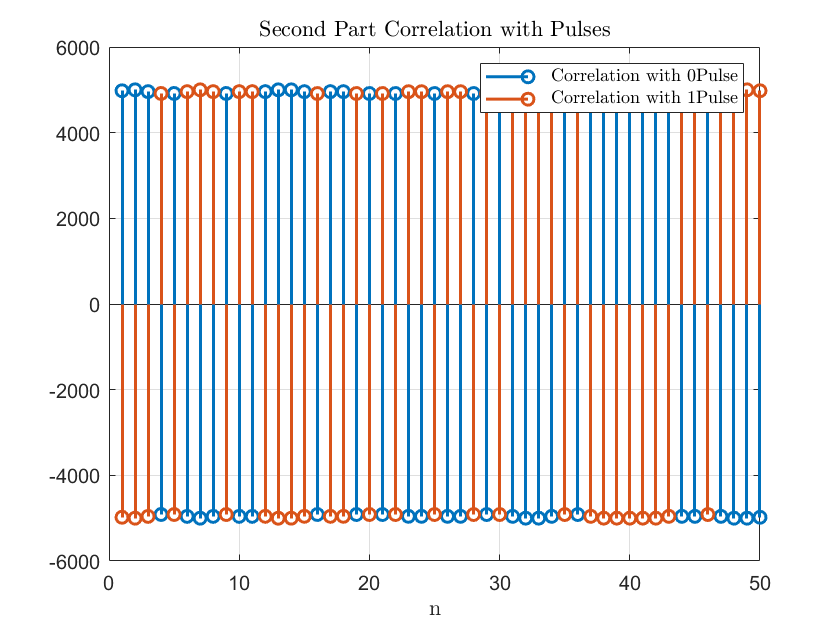
\includegraphics[width=0.4\textwidth]{comsys_fig12.png}\\ 
		\centering
	\end{figure}
	\begin{figure}[h!]
		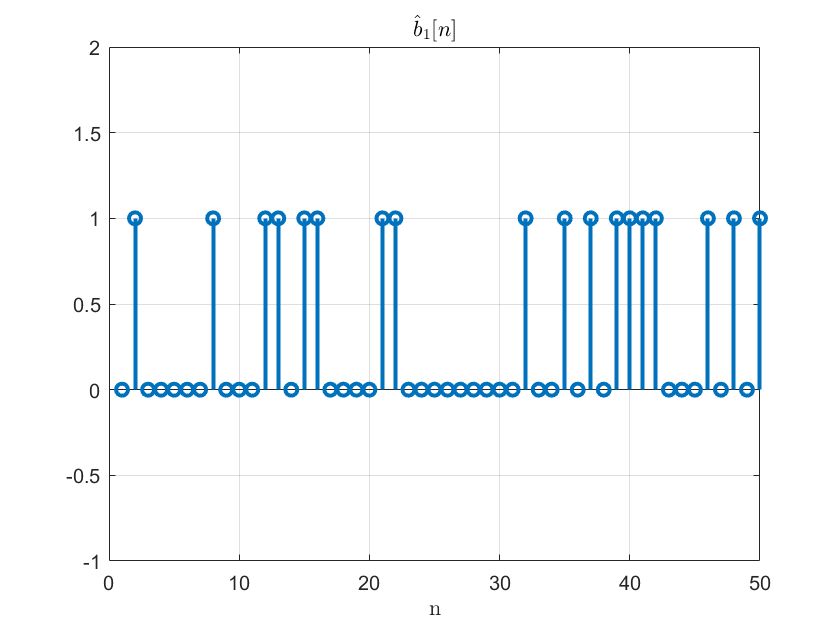
\includegraphics[width=0.5\textwidth]{comsys_fig13.png}\\ 
		\centering
	\end{figure}
	\begin{figure}[h!]
		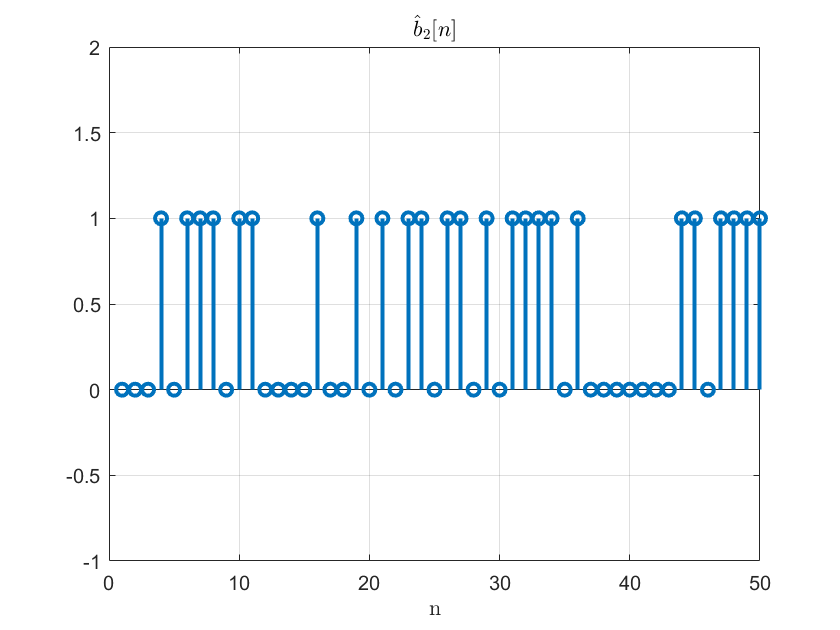
\includegraphics[width=0.5\textwidth]{comsys_fig14.png}\\ 
		\centering
	\end{figure}
	\newpage
	در نهایت با عبور از تابع \lr{Combine} خروجی را به دست می آوریم و آن را درکنار ورودی رسم می کنیم. میبینیم که درحالت بدون نویز سیستم ما بدون خطا کار می کند.
	\newline
	\begin{figure}[h!]
		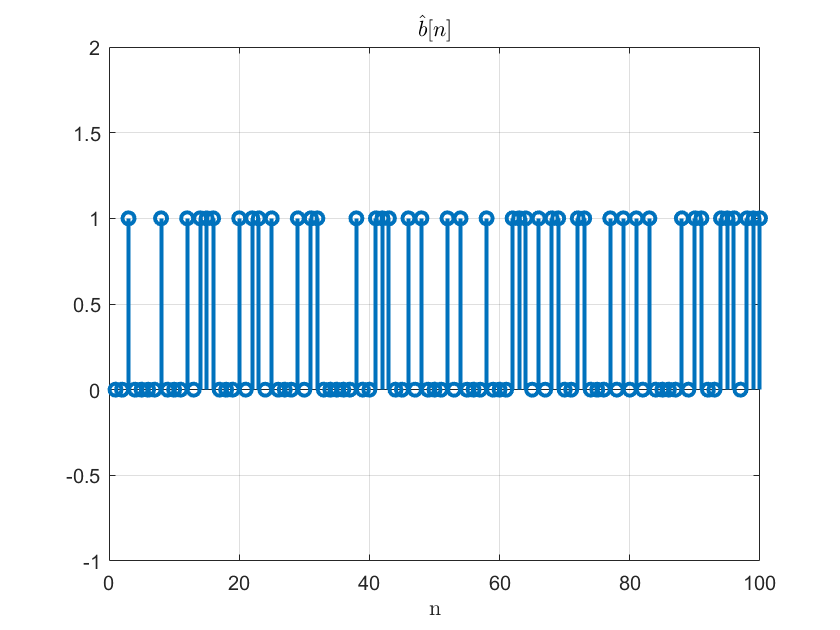
\includegraphics[width=0.5\textwidth]{comsys_fig15.png}\\ 
		\centering
	\end{figure}
	\begin{figure}[h!]
		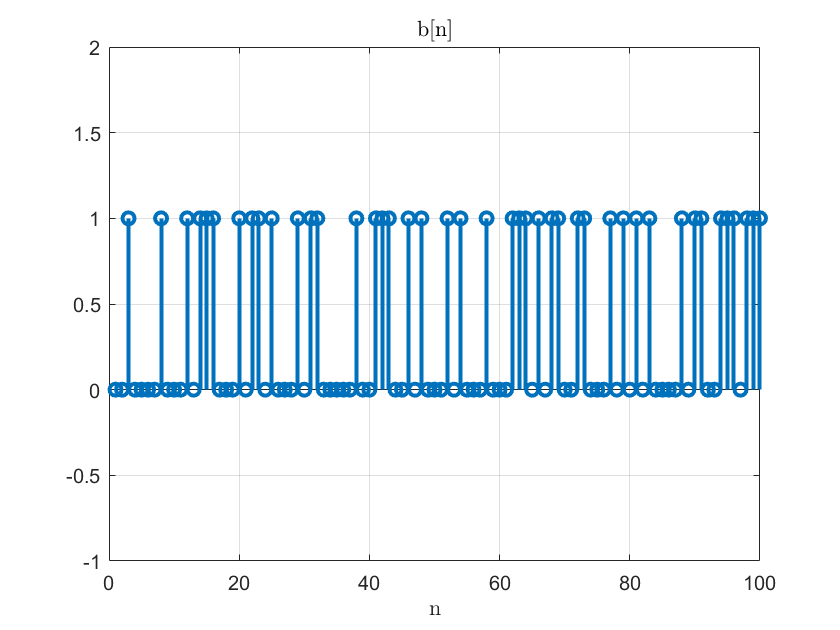
\includegraphics[width=0.5\textwidth]{comsys_fig16.png}\\ 
		\centering
	\end{figure}
	\newline
	\subsubsection*{ب}
	در این قسمت تابعی به نام \lr{DigitalSystem} پیاده شده که کل فرآیندهای قبل را به همراه نویز شبیه سازی می کند. به ازای مقادیر مختلف برای واریانس نویز یک نویز گاوسی به سیگنال 
	$y(t)$
	اضافه کرده و مقدار خطا را به دست می آوریم.
	\newline
	\begin{figure}[h!]
		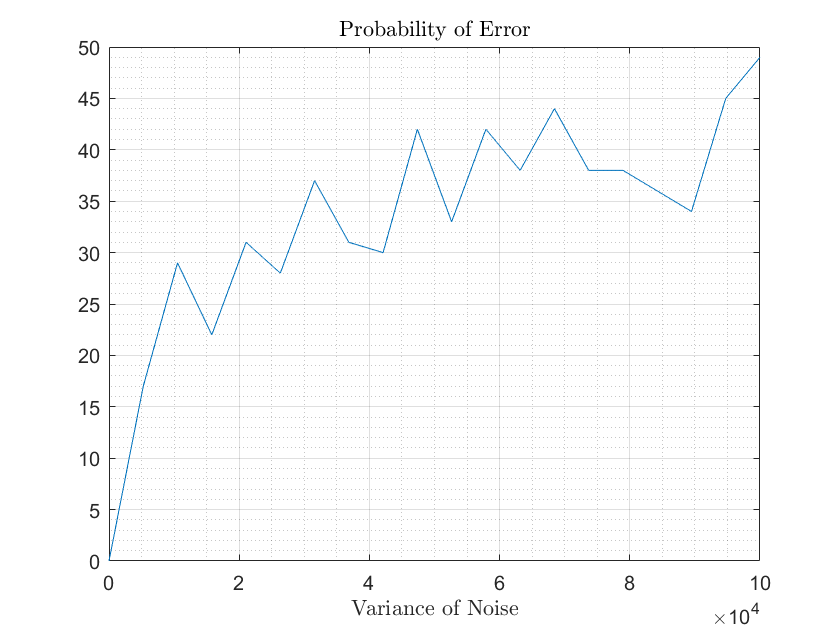
\includegraphics[width=0.5\textwidth]{comsys_fig17.png}\\ 
		\centering
	\end{figure}
	\newline
	مشاهده می شود که برای مقادیر بسیار زیاد واریانس ،احتمال خطا به حدود 50 درصد می رسد!
	\subsubsection*{ج}
	به ازای 6 مقدار مختلف برای واریانس نویز \lr{Signal Constellation} را رسم می کنیم.
	\newline
	\begin{figure}[h!]
		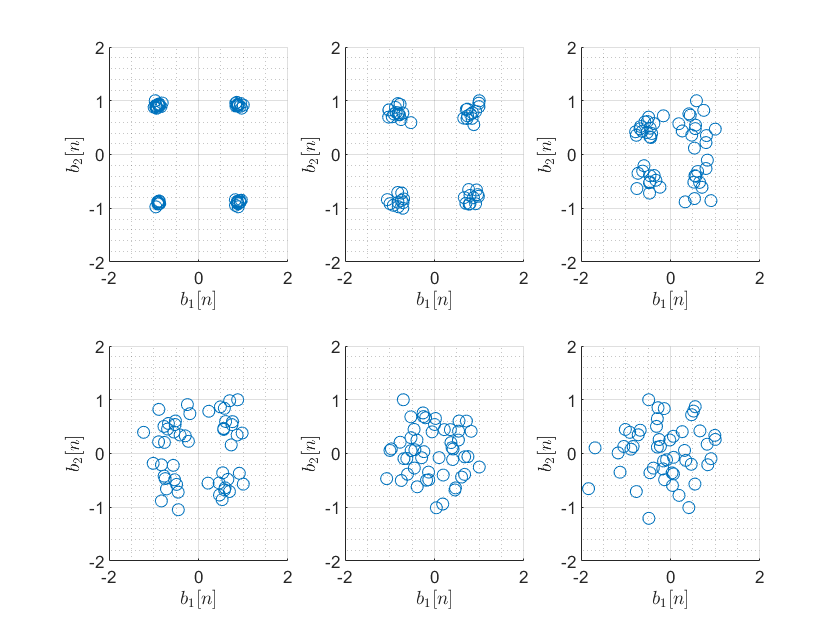
\includegraphics[width=0.8\textwidth]{comsys_fig18.png}\\ 
		\centering
	\end{figure}
	\newline
	در نمودارهای بالا مقادیر حاصل از \lr{Matched Filter} نرمالیزه شده اند تا نقاط حول نقطه های 
	$\pm 1$
	متمرکز شوند. می توان مشاهده کرد که با افزایش واریانس پراکندگی نقاط بیشتر میشود و در نتیجه احتمال خطا هم افزایش پیدا خواهد کرد.
	\subsection{مدولاسیون \lr{PSK}}
	\subsubsection*{الف}
	همانند قسمت قبل برای این بخش هم سیگنال ها را به دست آورده و رسم می کنیم.می توان مشاهده کرد که در این حالت هم در حالت بدون نویز سیگنال بدون خطا انتقال می یابد.
	\newline
	\begin{figure}[H]
		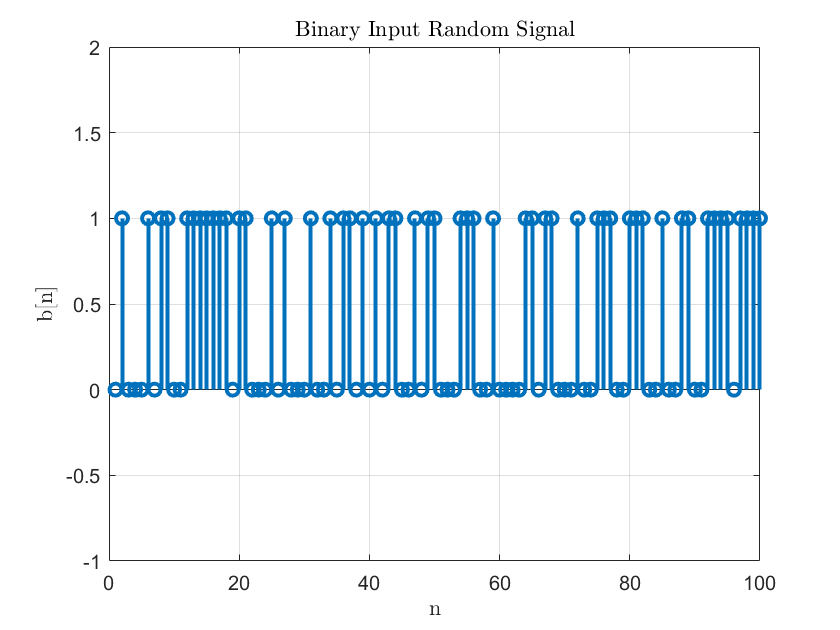
\includegraphics[width=0.4\textwidth]{comsys_fig19.png}\\ 
		\centering
	\end{figure}\begin{figure}[H]
	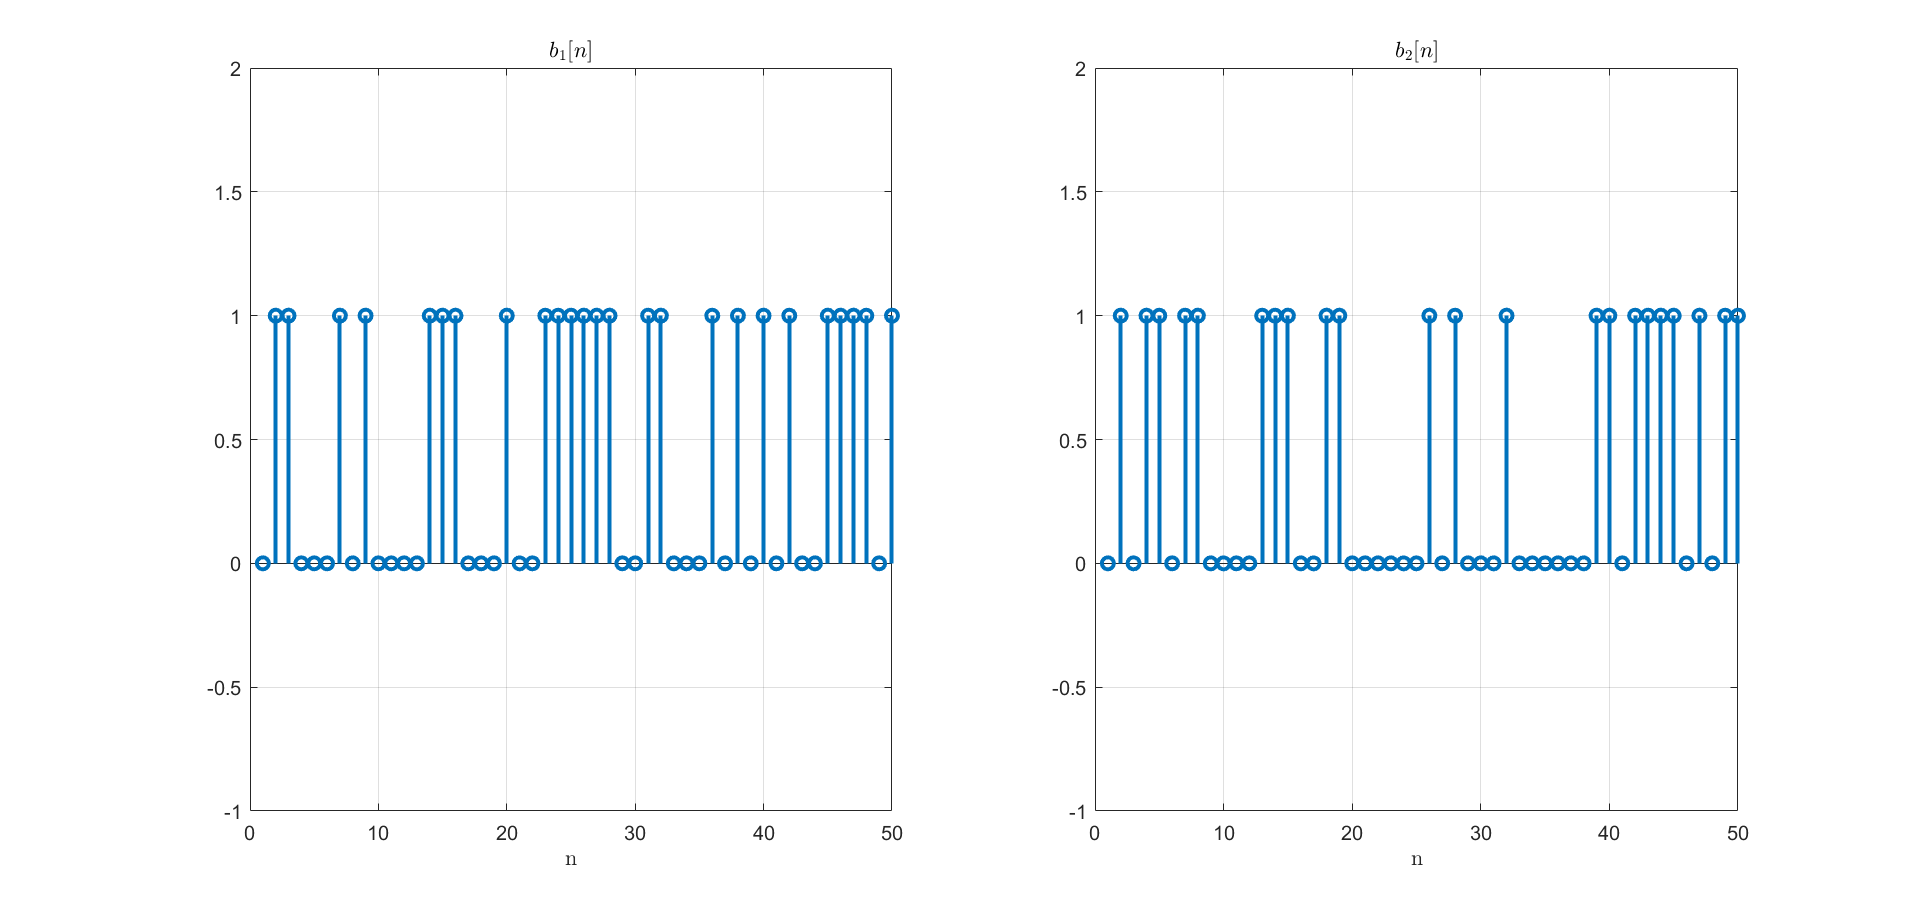
\includegraphics[width=0.8\textwidth]{comsys_fig20.png}\\ 
	\centering
	\end{figure}\begin{figure}[H]
	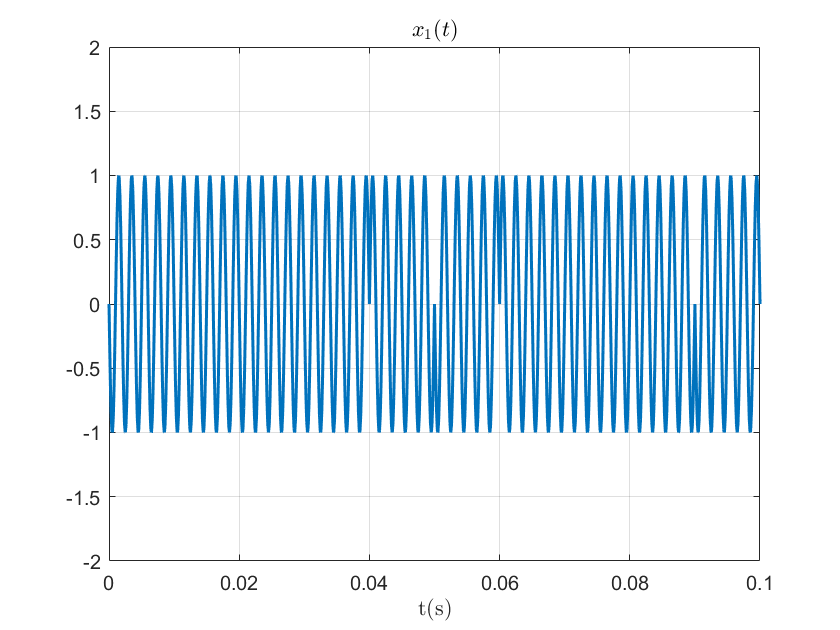
\includegraphics[width=0.6\textwidth]{comsys_fig21.png}\\ 
	\centering
	\end{figure}\begin{figure}[H]
	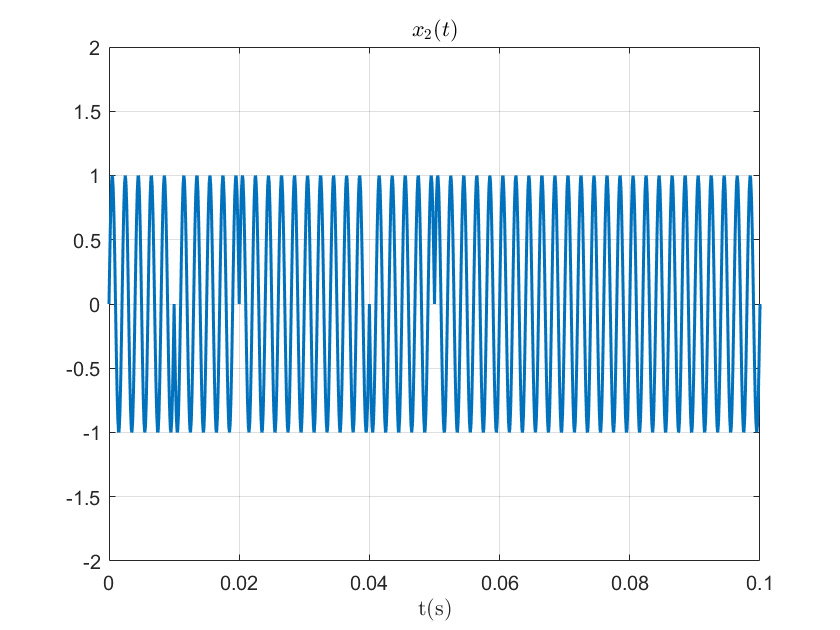
\includegraphics[width=0.6\textwidth]{comsys_fig22.png}\\ 
	\centering
	\end{figure}
	\begin{figure}[H]
		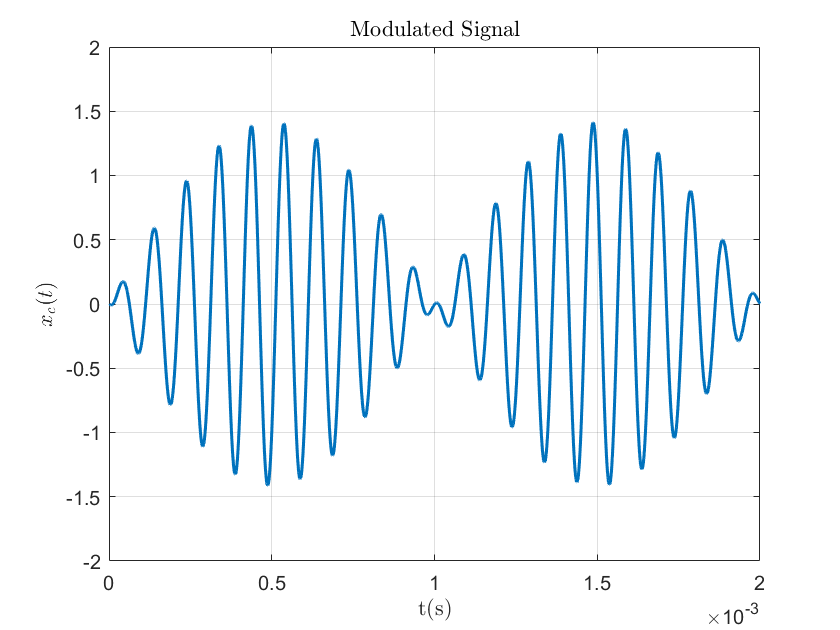
\includegraphics[width=0.5\textwidth]{comsys_fig23.png}\\ 
		\centering
	\end{figure}\begin{figure}[H]
	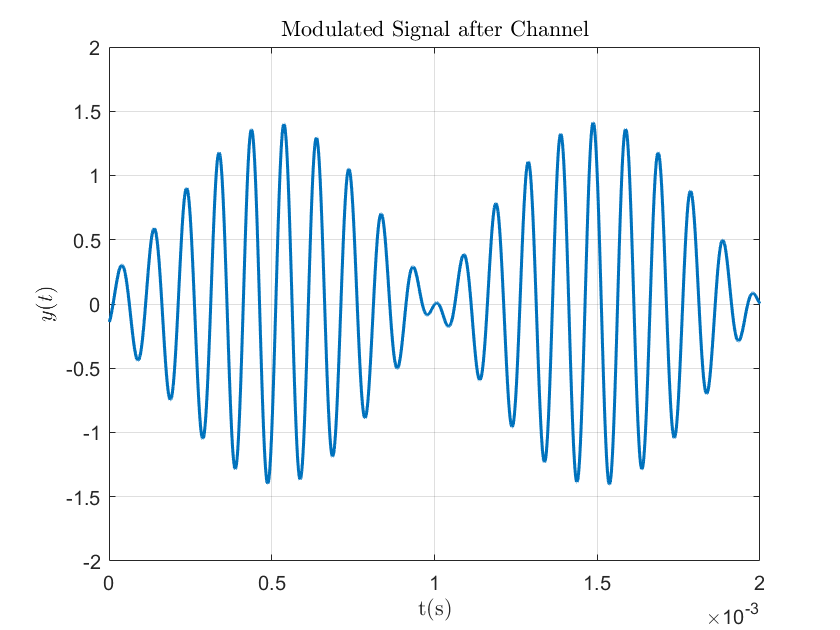
\includegraphics[width=0.6\textwidth]{comsys_fig24.png}\\ 
	\centering
	\end{figure}\begin{figure}[H]
	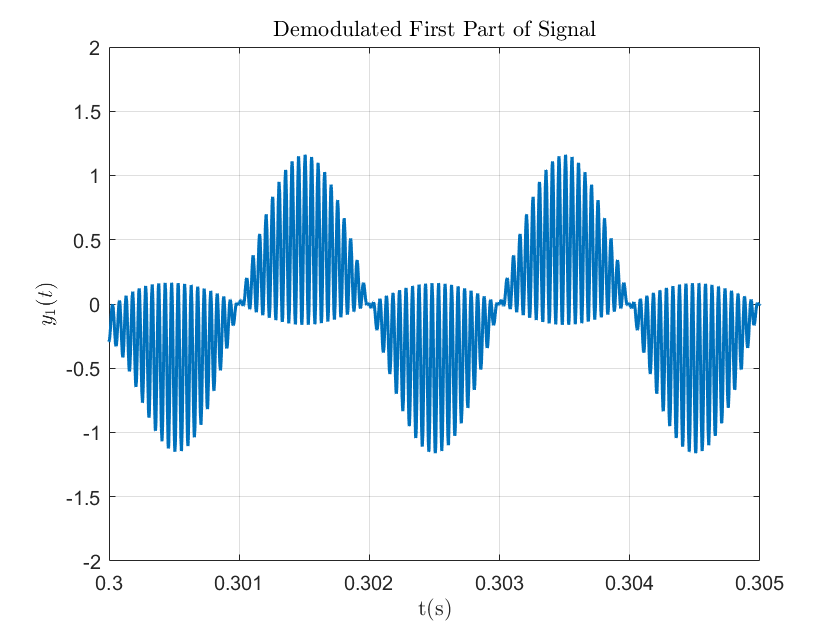
\includegraphics[width=0.6\textwidth]{comsys_fig25.png}\\ 
	\centering
	\end{figure}\begin{figure}[H]
	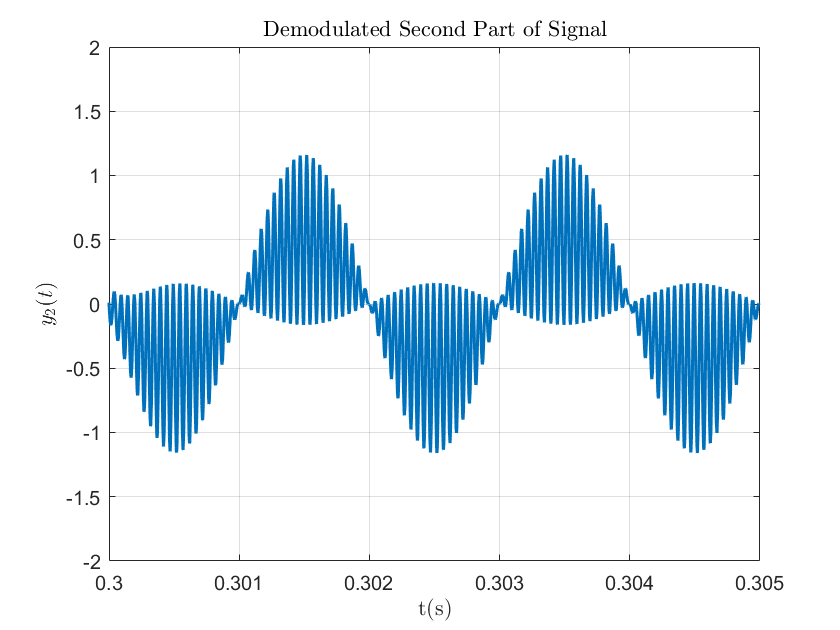
\includegraphics[width=0.4\textwidth]{comsys_fig26.png}\\ 
	\centering
	\end{figure}\begin{figure}[H]
	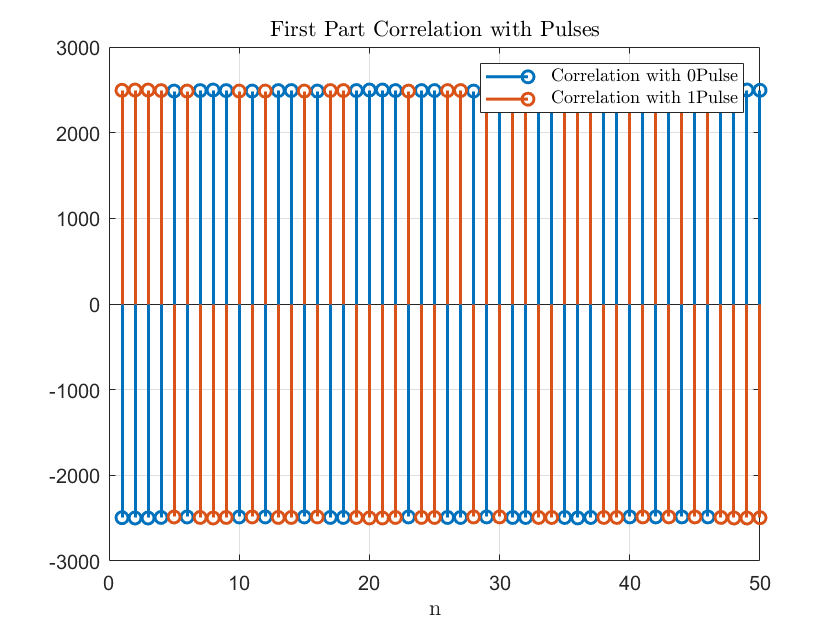
\includegraphics[width=0.4\textwidth]{comsys_fig27.png}\\ 
	\centering
	\end{figure}\begin{figure}[H]
	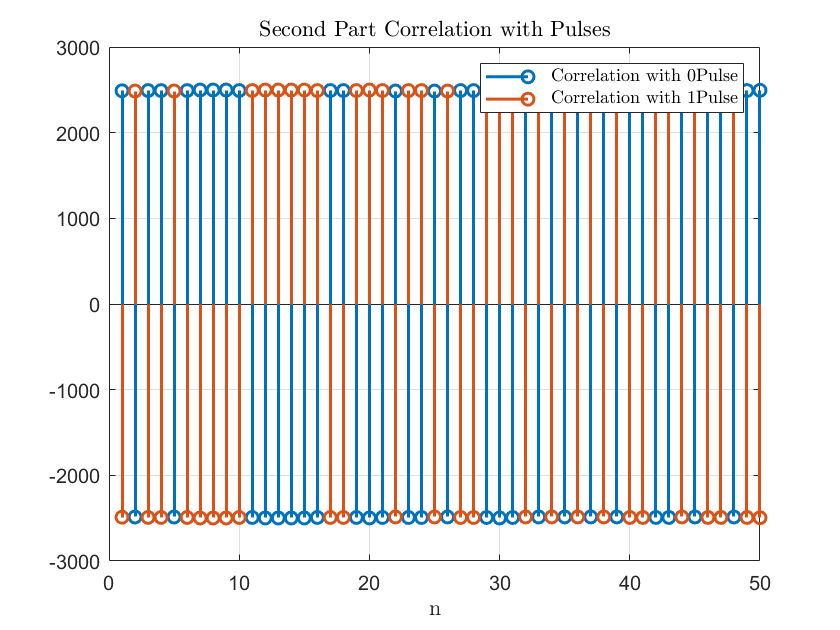
\includegraphics[width=0.4\textwidth]{comsys_fig28.png}\\ 
	\centering
	\end{figure}\begin{figure}[H]
	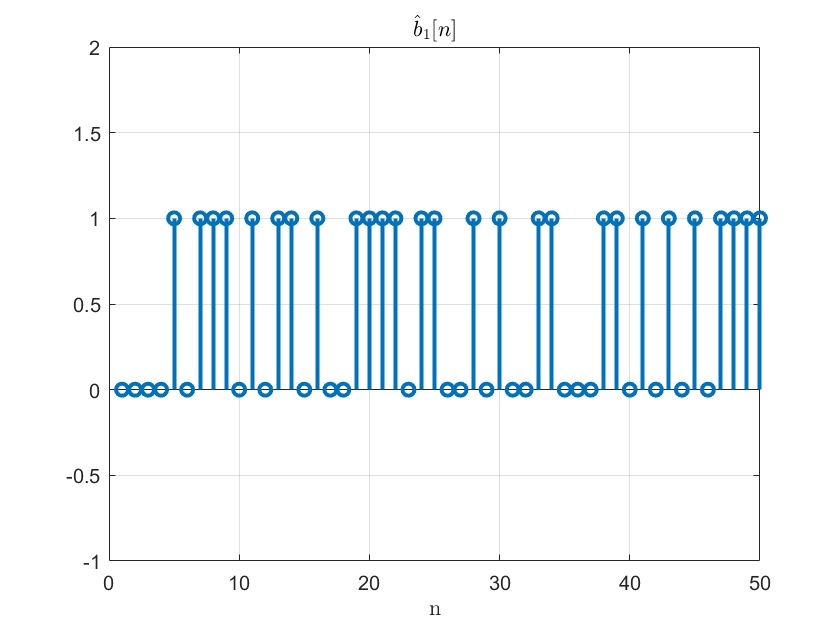
\includegraphics[width=0.45\textwidth]{comsys_fig29.png}\\ 
	\centering
	\end{figure}\begin{figure}[H]
	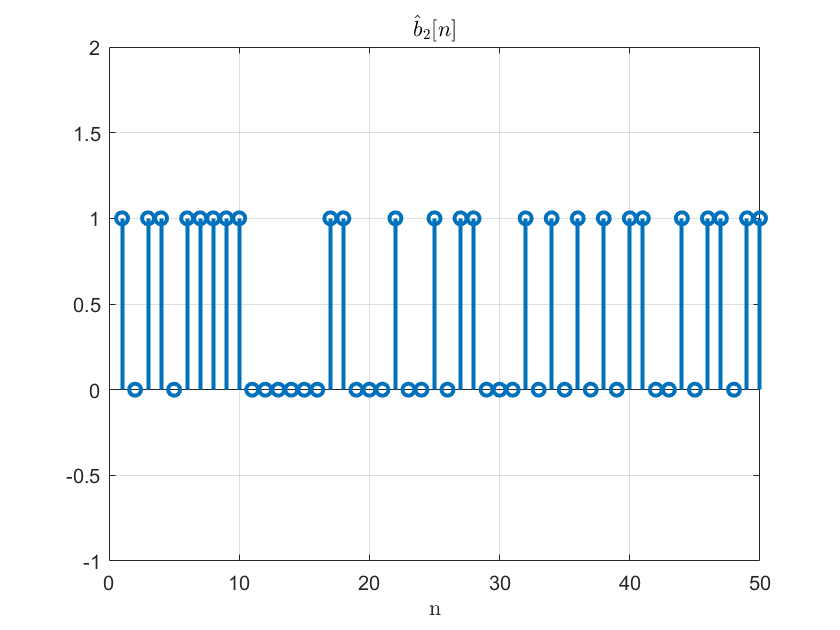
\includegraphics[width=0.55\textwidth]{comsys_fig30.png}\\ 
	\centering
	\end{figure}\begin{figure}[H]
	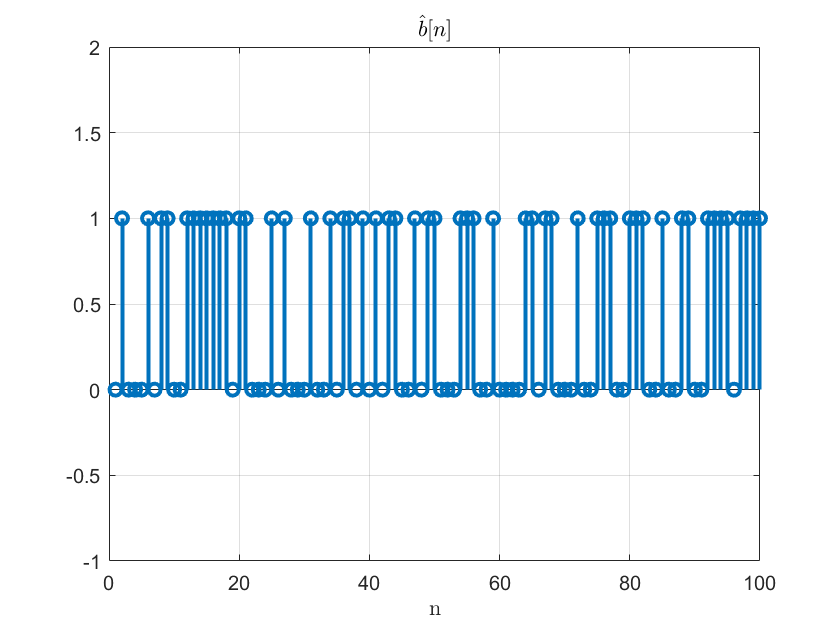
\includegraphics[width=0.55\textwidth]{comsys_fig31.png}\\ 
	\centering
	\end{figure}\begin{figure}[H]
	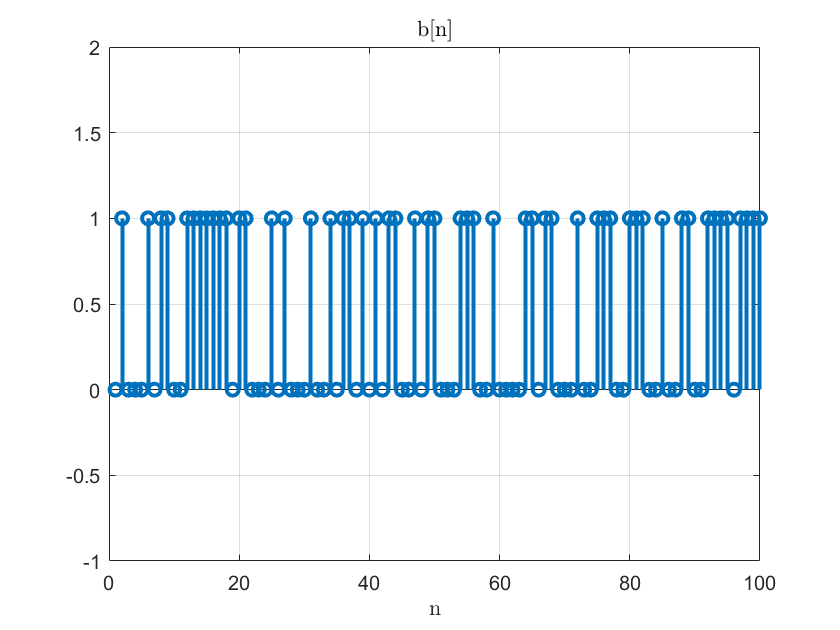
\includegraphics[width=0.55\textwidth]{comsys_fig32.png}\\ 
	\centering
	\end{figure}
	\subsubsection*{ب}
	می توان مشاهده کرد که همانند حالت قبل به ازای مقادیر خیلی بزرگ واریانس ، خطا به حدود 50 درصد می رسد.
	\newline
	\begin{figure}[H]
		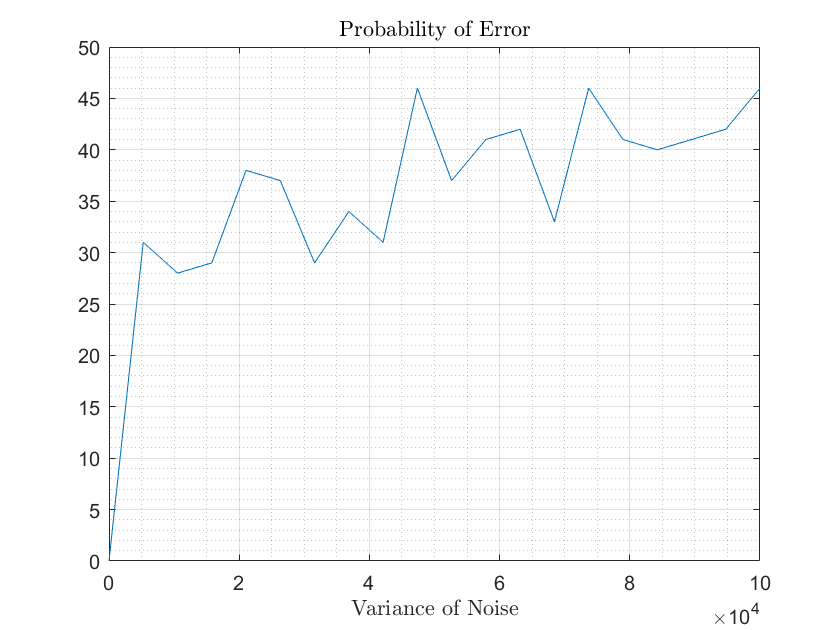
\includegraphics[width=0.5\textwidth]{comsys_fig33.png}\\ 
		\centering
	\end{figure}
	\subsubsection*{ج}
	می بینیم که همانند حالت قبل با افزایش واریانس پراکندگی افزایش یافته و احتمال خطا بیشتر می شود.
	\begin{figure}[H]
		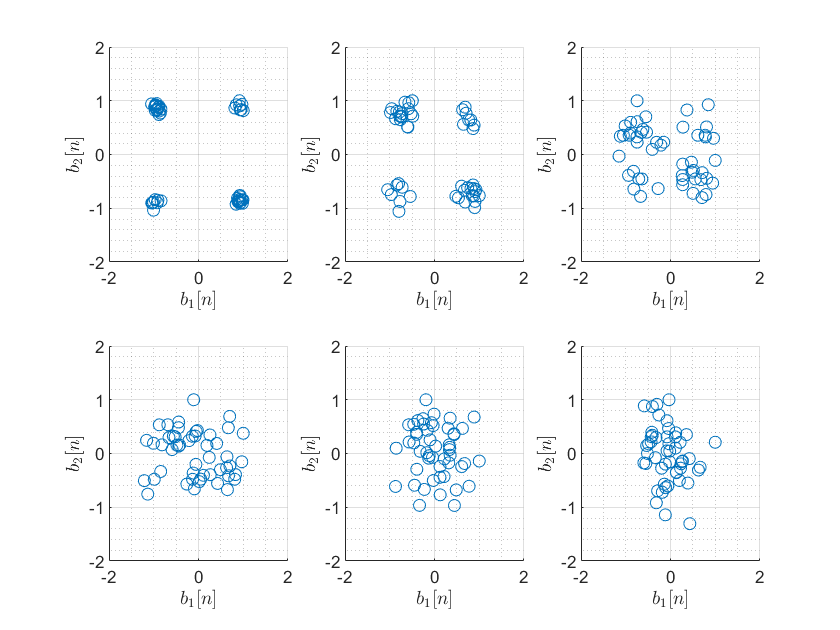
\includegraphics[width=0.8\textwidth]{comsys_fig34.png}\\ 
		\centering
	\end{figure}
	\subsection{مدولاسیون \lr{FSK}}
	\subsubsection*{الف}
	بله دو سیگنال متعامد هستند و تعامد آنها به این صورت اثبات می شود:
	\begin{equation*}
		P_0 = \sin (2 \pi 1000 t)
	\end{equation*}
	\begin{equation*}
		P_1 = \sin (2 \pi 1500 t)
	\end{equation*}
	\begin{equation*}
		\big<P_0 , P_1\big> = \int_{0}^{T} \sin (2 \pi 1000 t) \sin (2 \pi 1500 t) dt = 0 
	\end{equation*}
	\subsubsection*{ب}
	همانند حالت های قبل سیگنال ها را رسم می کنیم
	\begin{figure}[H]
		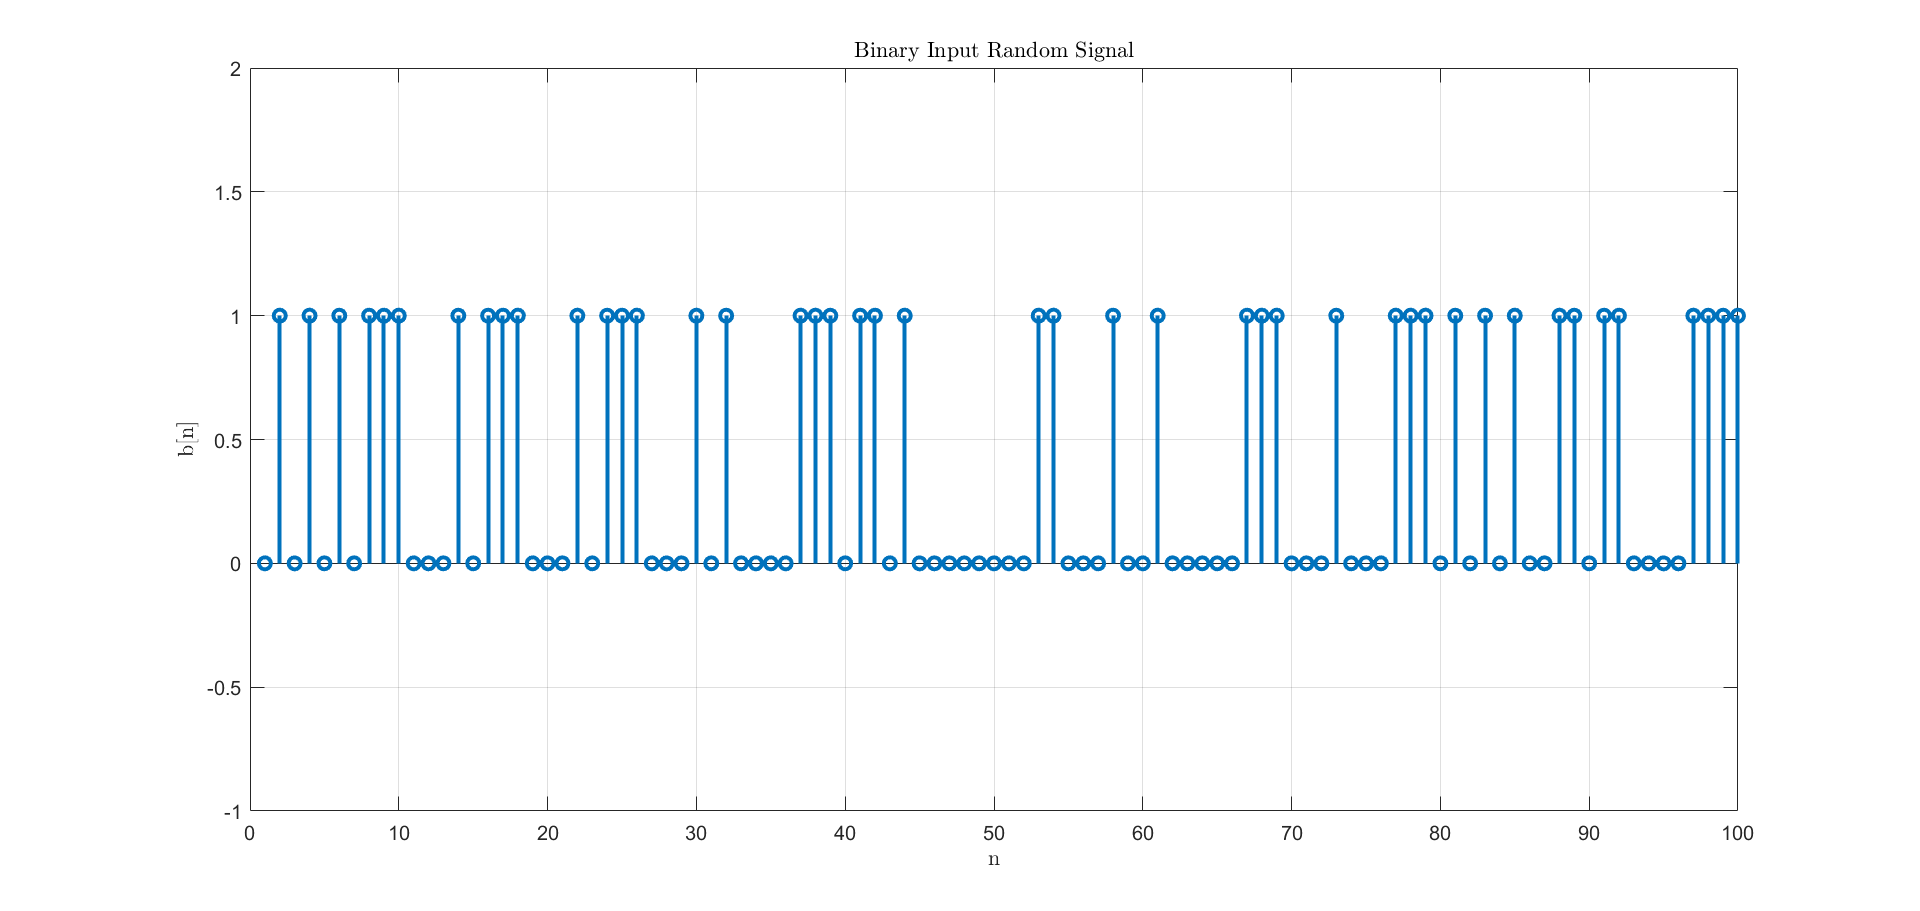
\includegraphics[width=0.8\textwidth]{comsys_fig35.png}\\ 
		\centering
	\end{figure}
	\begin{figure}[H]
		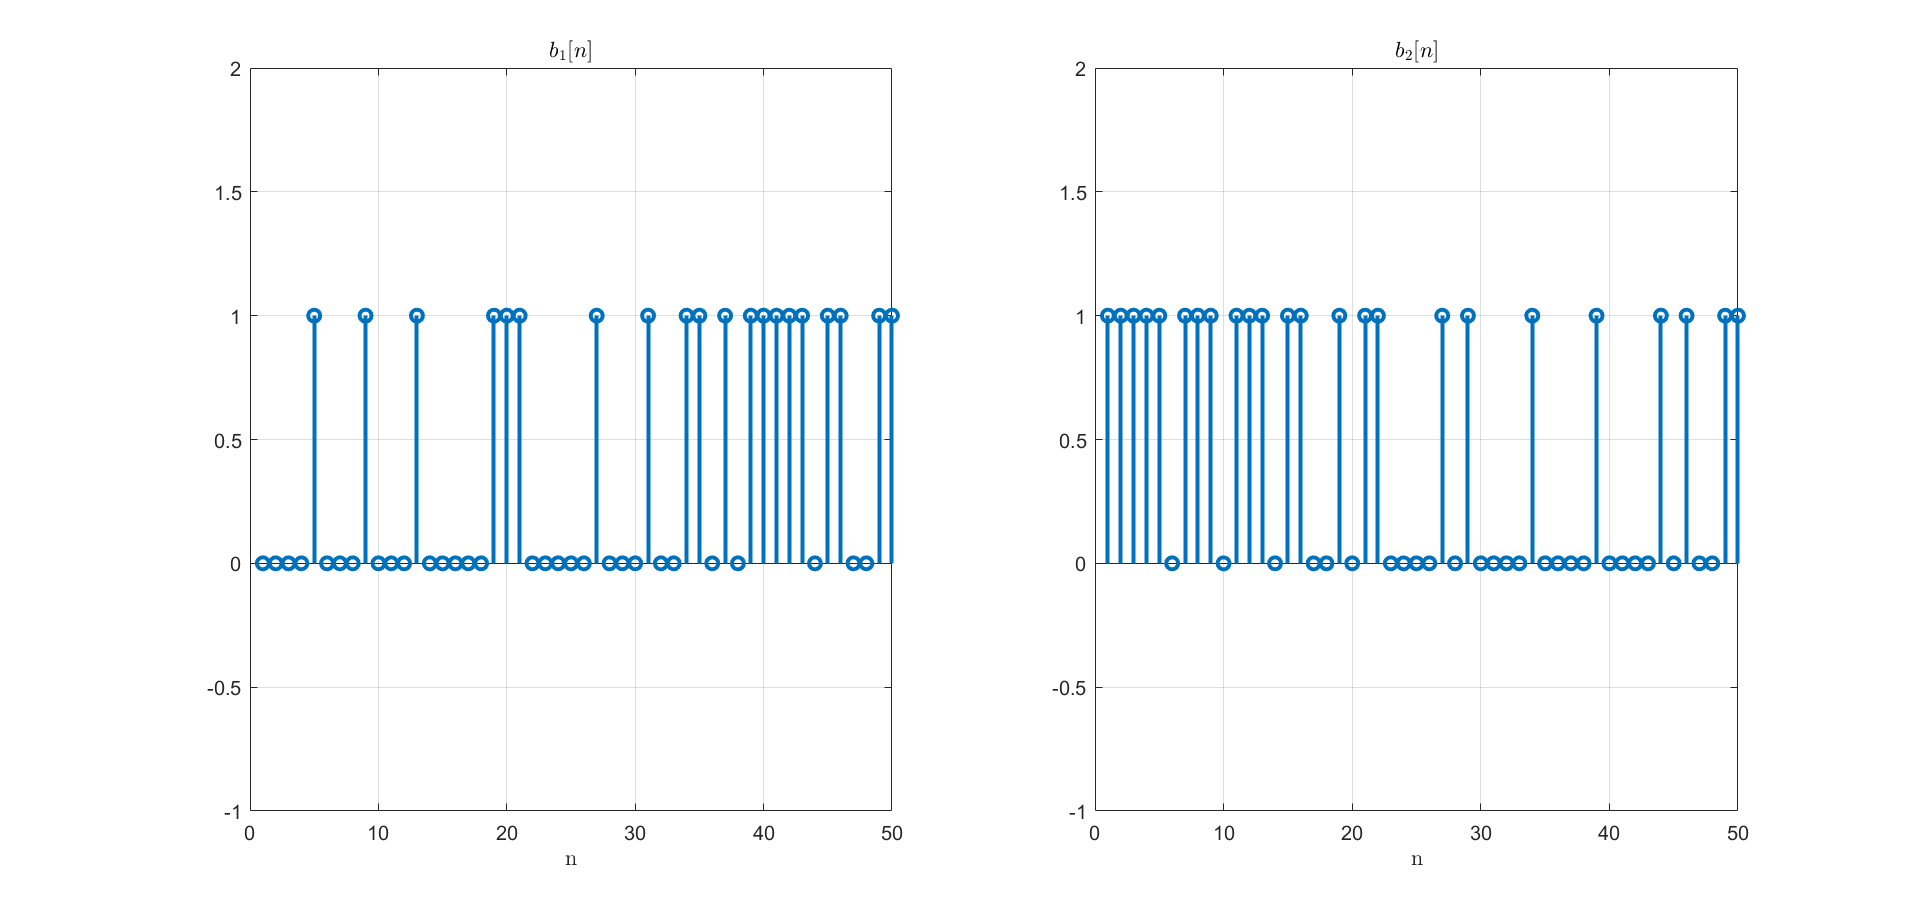
\includegraphics[width=0.8\textwidth]{comsys_fig36.png}\\ 
		\centering
	\end{figure}
	\begin{figure}[H]
		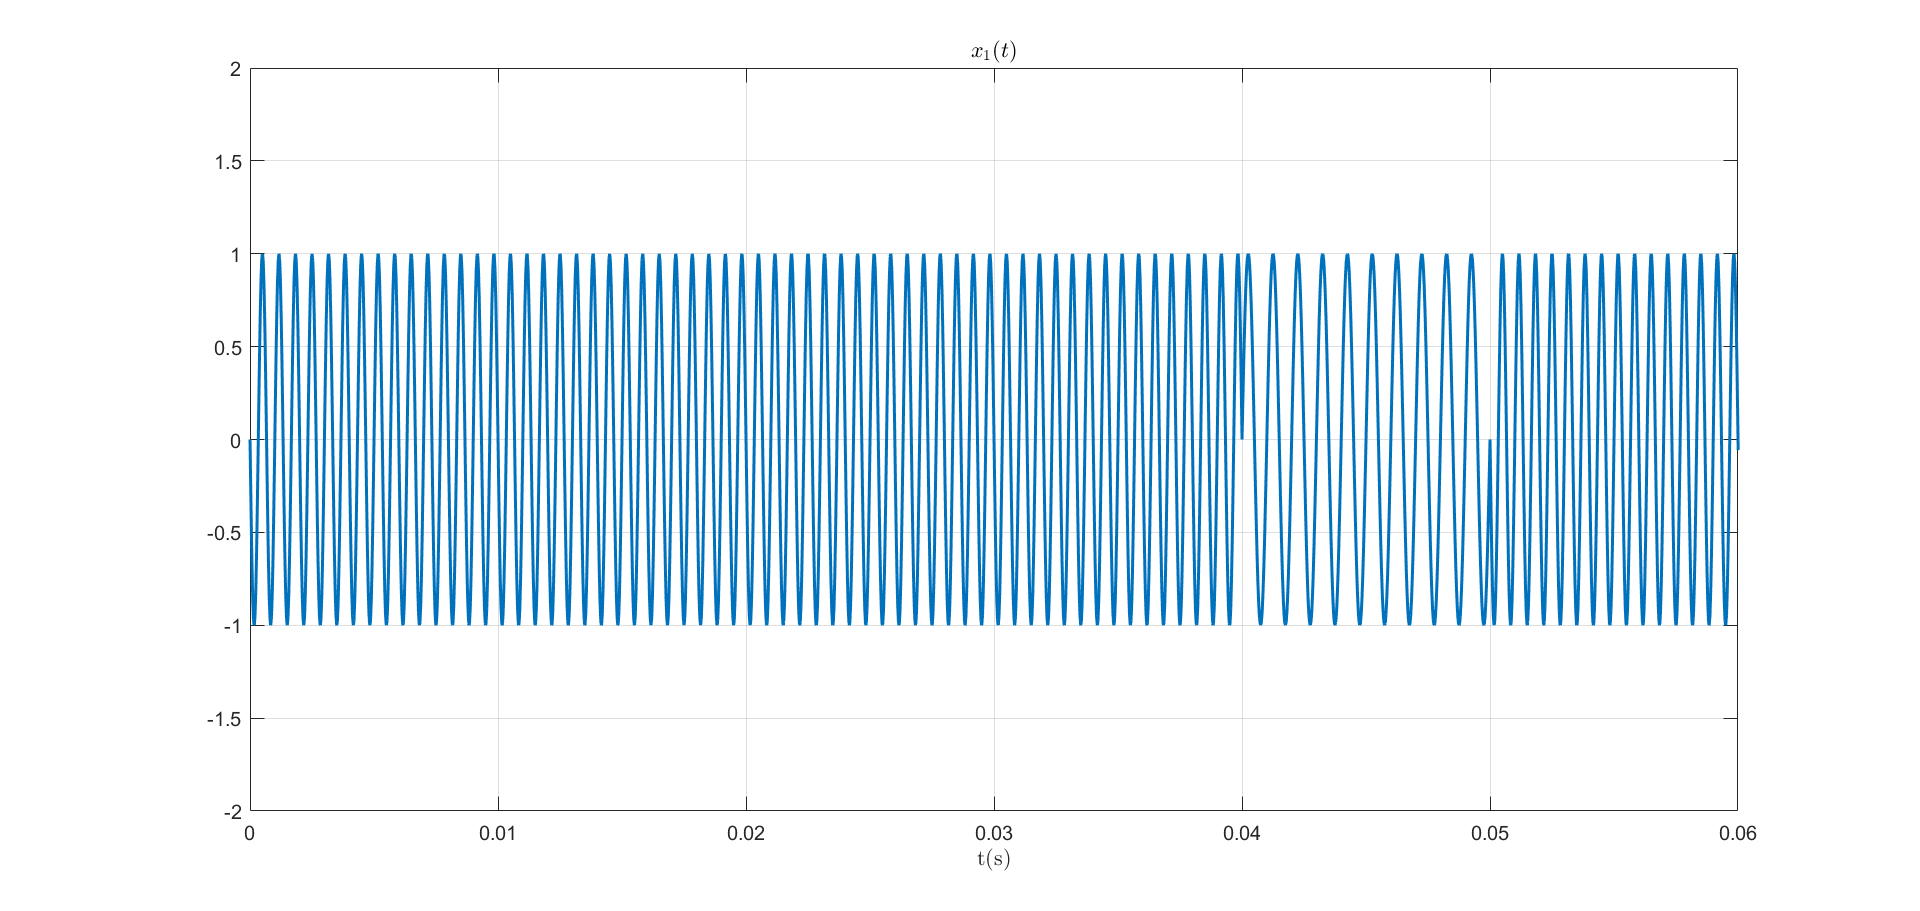
\includegraphics[width=0.8\textwidth]{comsys_fig37.png}\\ 
		\centering
	\end{figure}
	\begin{figure}[H]
		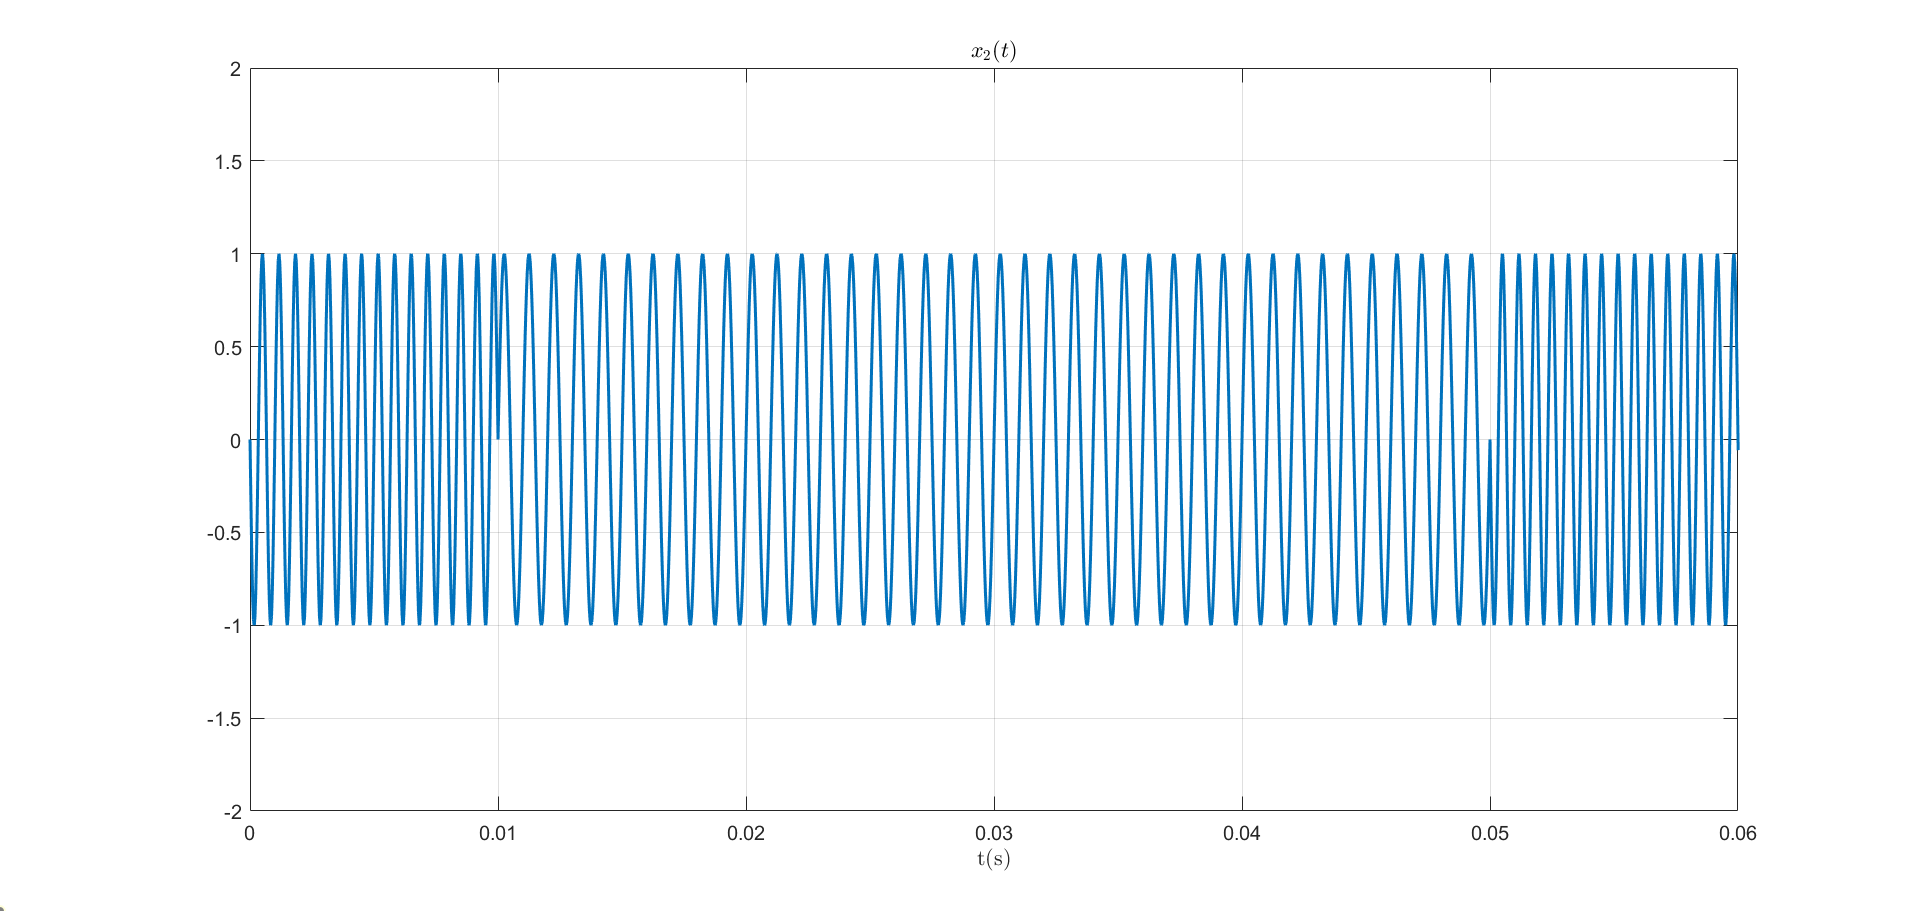
\includegraphics[width=0.8\textwidth]{comsys_fig38.png}\\ 
		\centering
	\end{figure}
	\begin{figure}[H]
		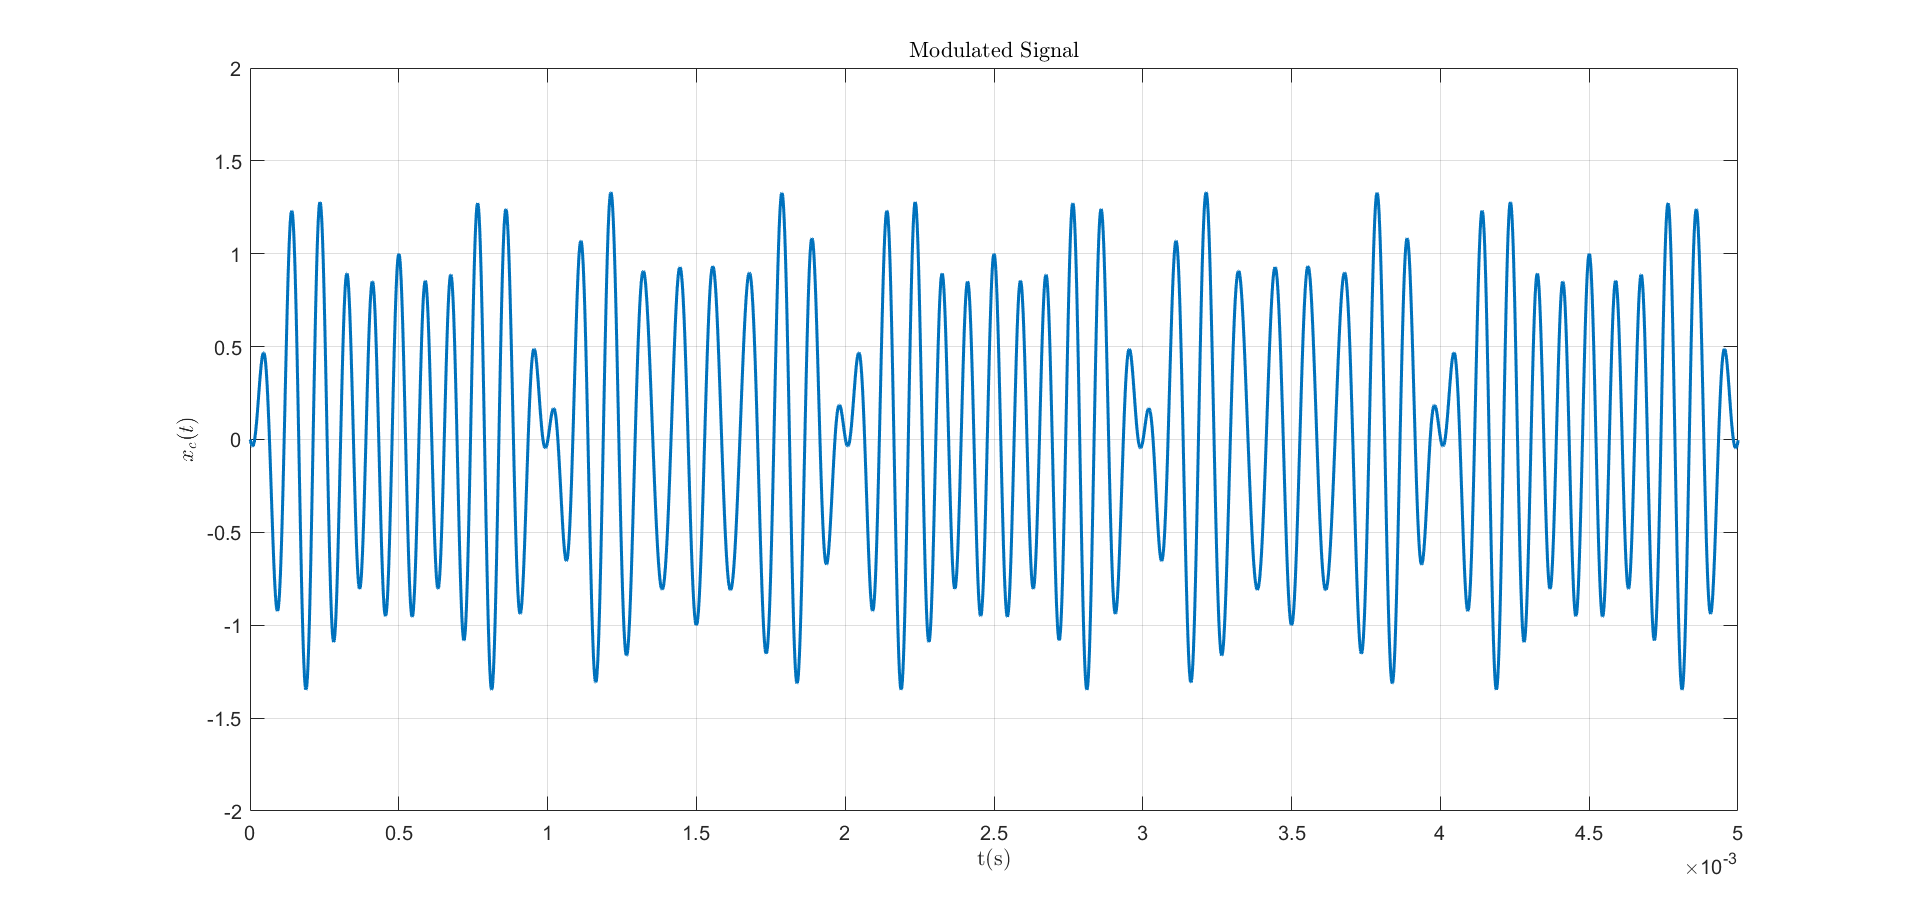
\includegraphics[width=0.8\textwidth]{comsys_fig39.png}\\ 
		\centering
	\end{figure}
	\begin{figure}[H]
		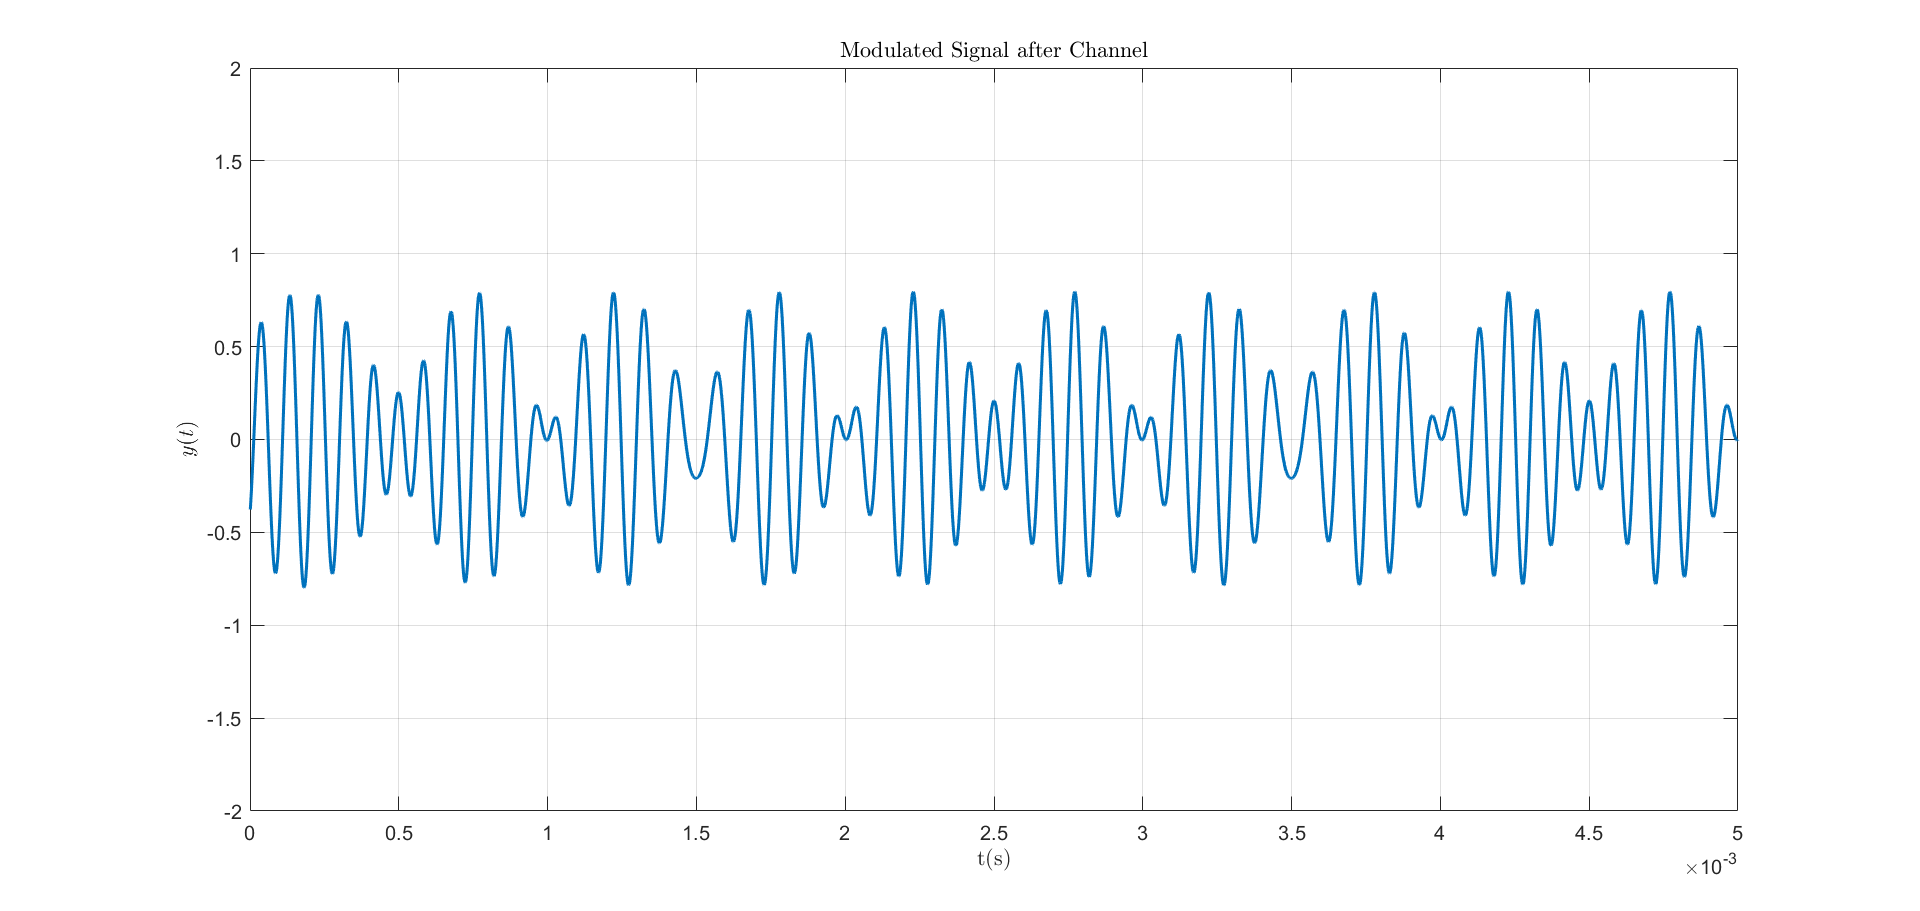
\includegraphics[width=0.8\textwidth]{comsys_fig40.png}\\ 
		\centering
	\end{figure}
	\begin{figure}[H]
		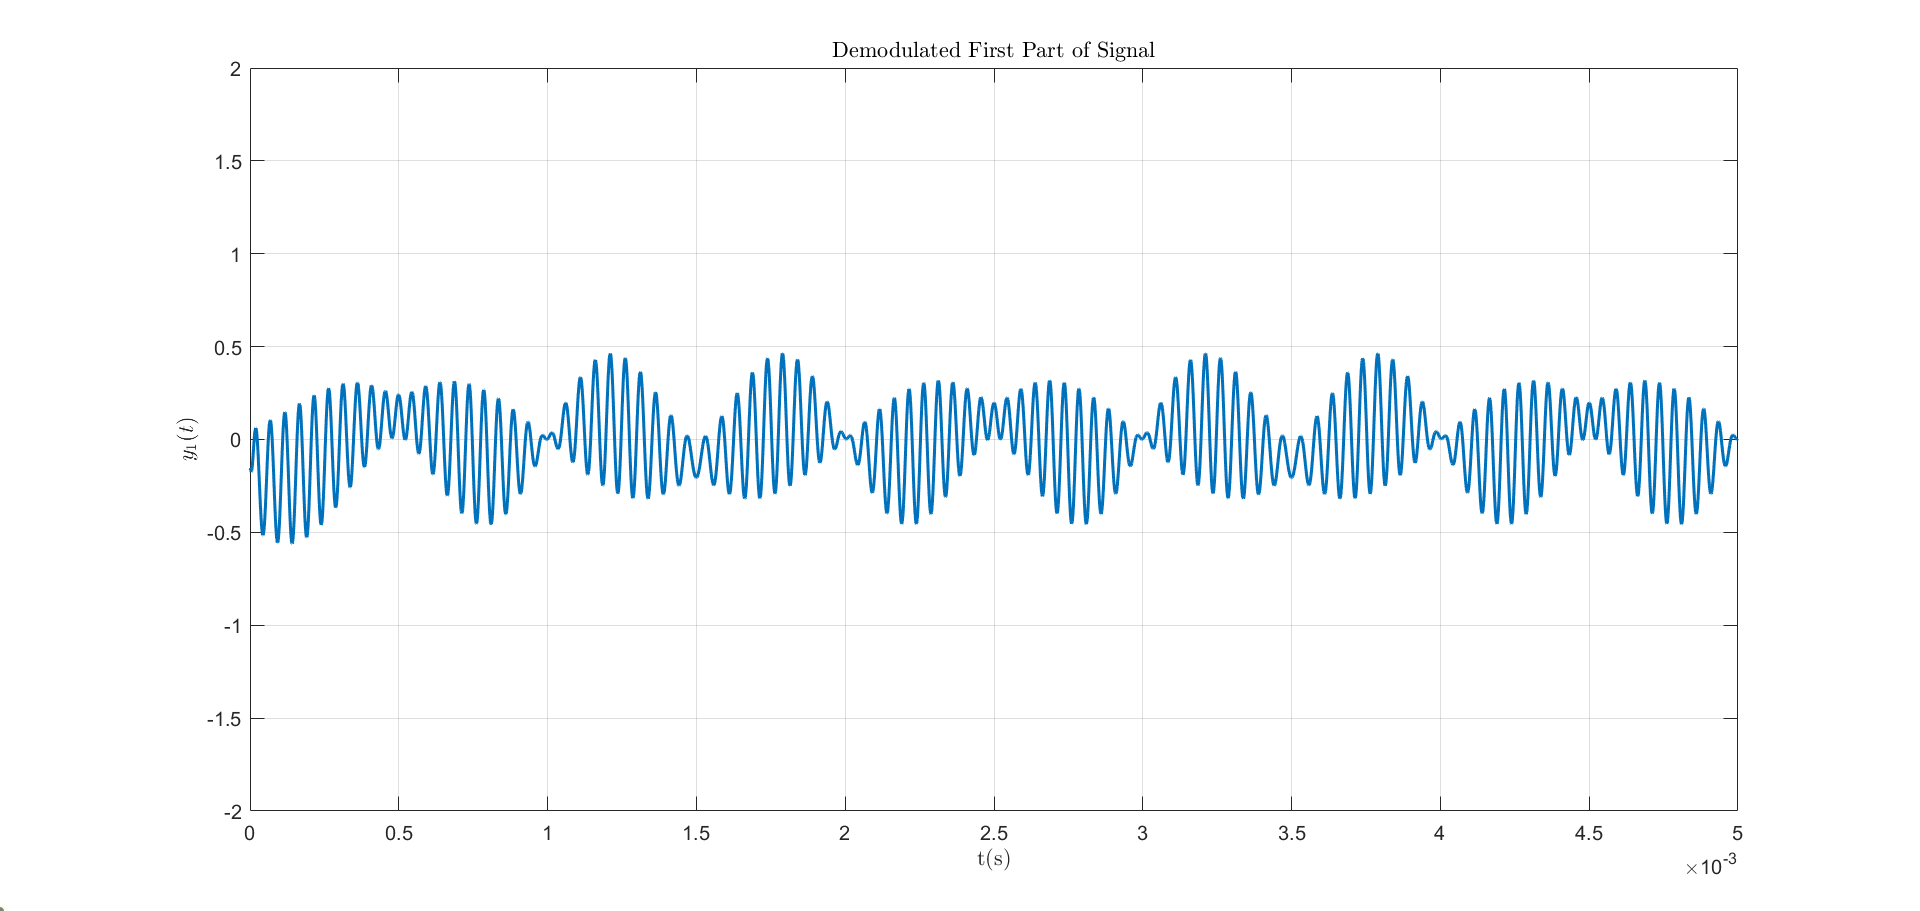
\includegraphics[width=0.8\textwidth]{comsys_fig41.png}\\ 
		\centering
	\end{figure}
	\begin{figure}[H]
		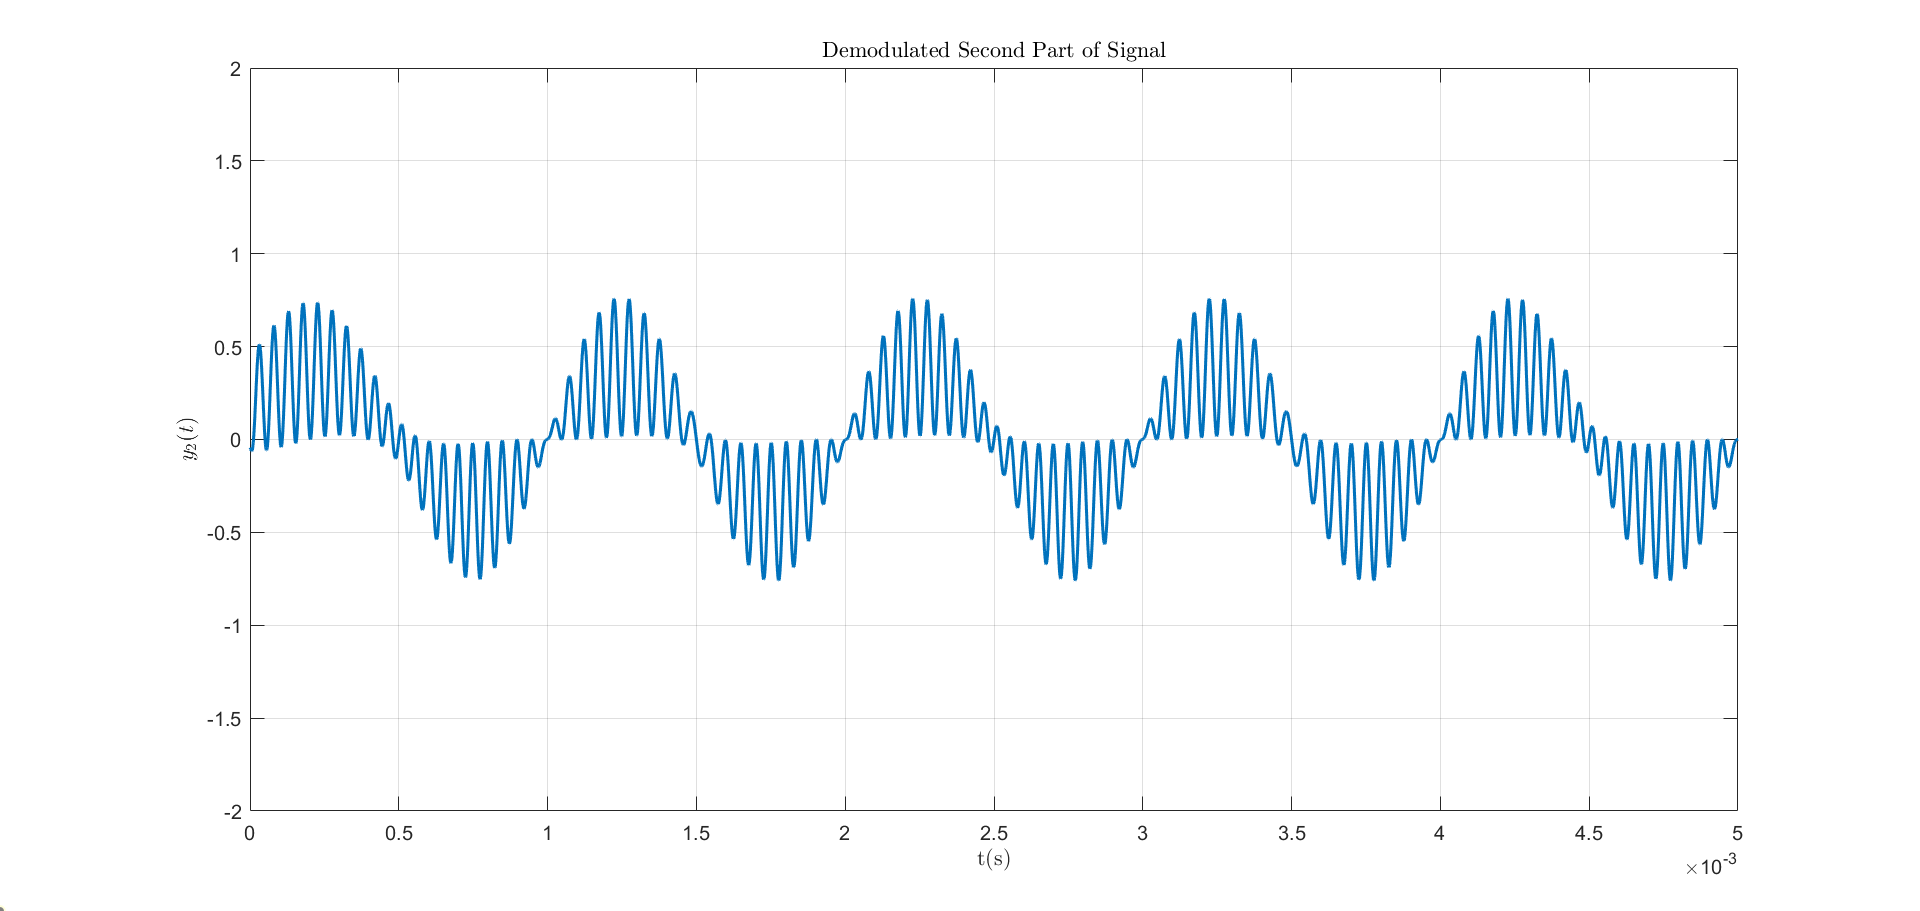
\includegraphics[width=0.8\textwidth]{comsys_fig42.png}\\ 
		\centering
	\end{figure}
	\begin{figure}[H]
		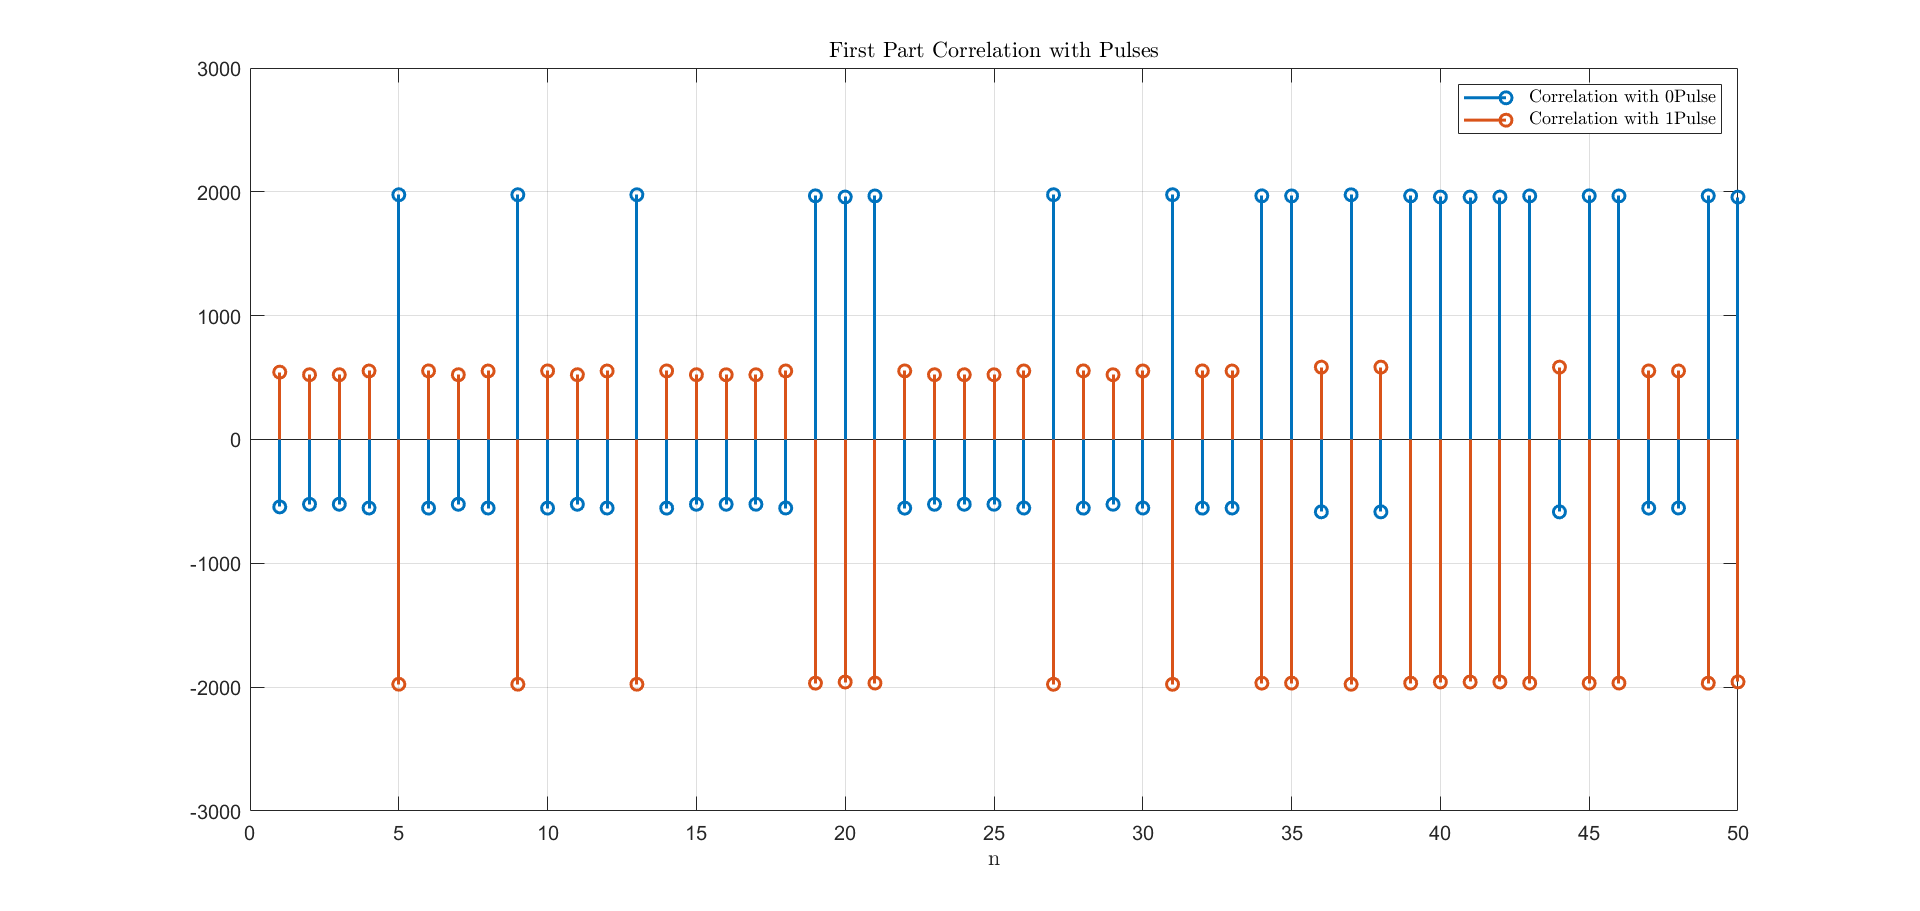
\includegraphics[width=0.8\textwidth]{comsys_fig43.png}\\ 
		\centering
	\end{figure}
	\begin{figure}[H]
		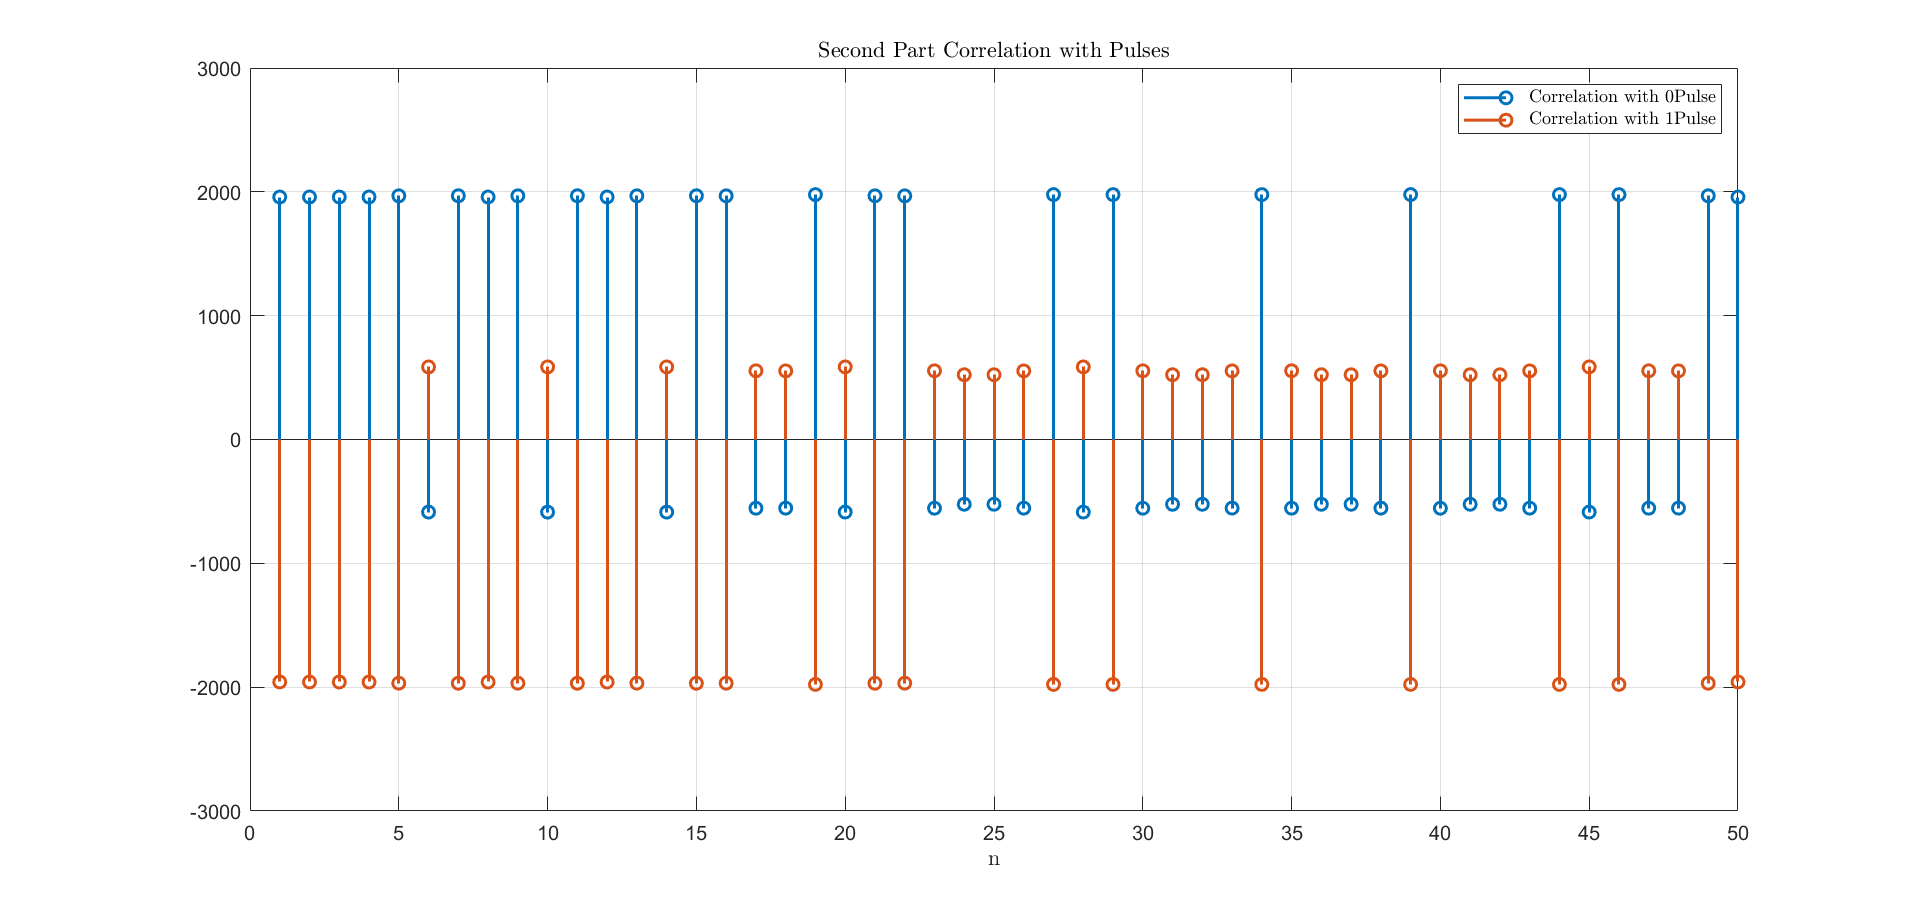
\includegraphics[width=0.8\textwidth]{comsys_fig44.png}\\ 
		\centering
	\end{figure}
	\begin{figure}[H]
		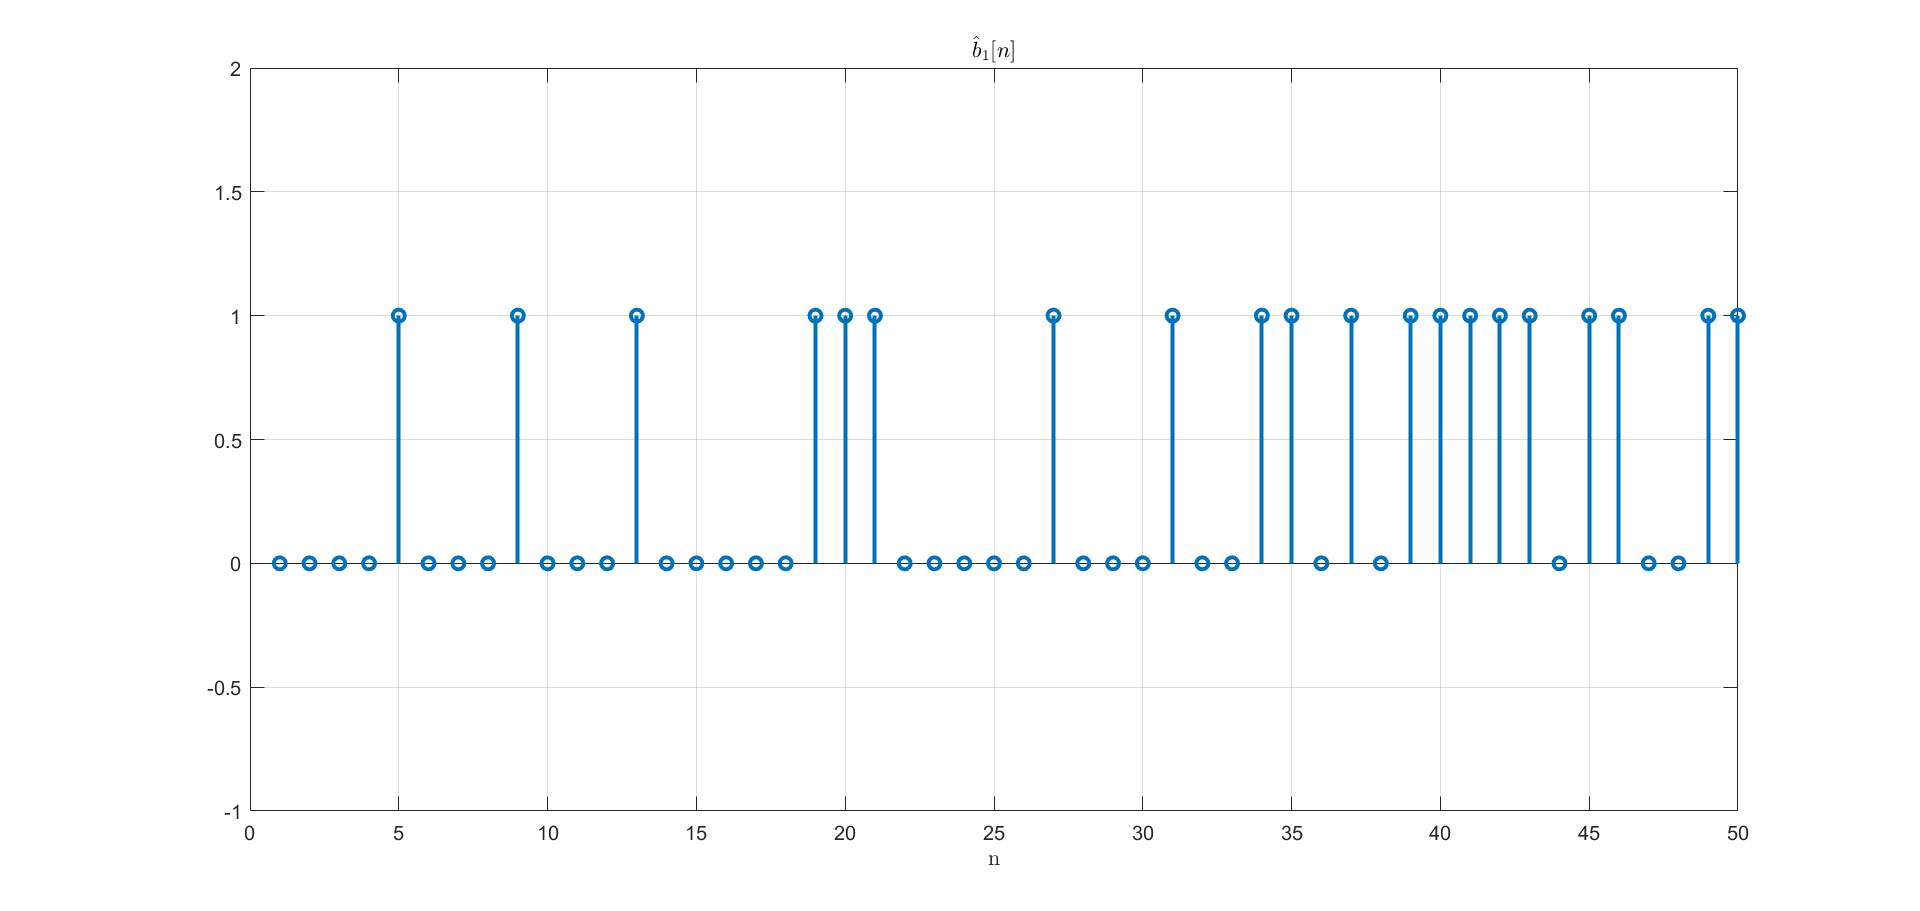
\includegraphics[width=0.8\textwidth]{comsys_fig45.png}\\ 
		\centering
	\end{figure}
	\begin{figure}[H]
		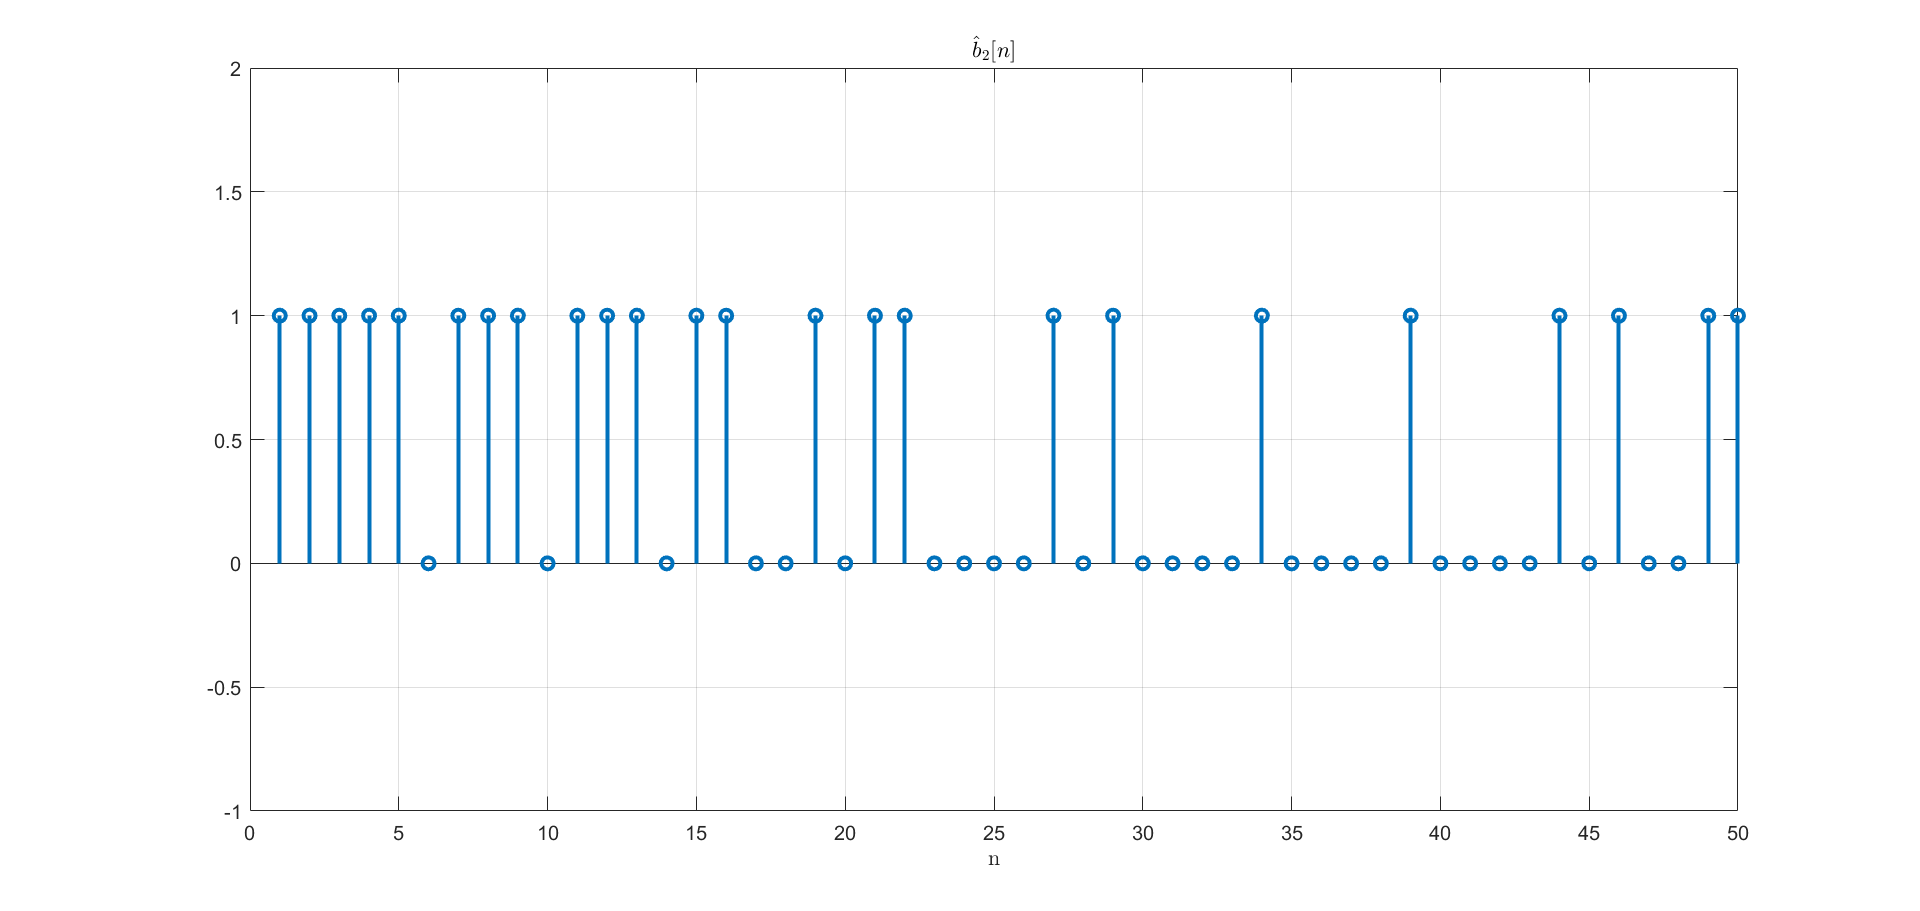
\includegraphics[width=0.8\textwidth]{comsys_fig46.png}\\ 
		\centering
	\end{figure}
	\begin{figure}[H]
		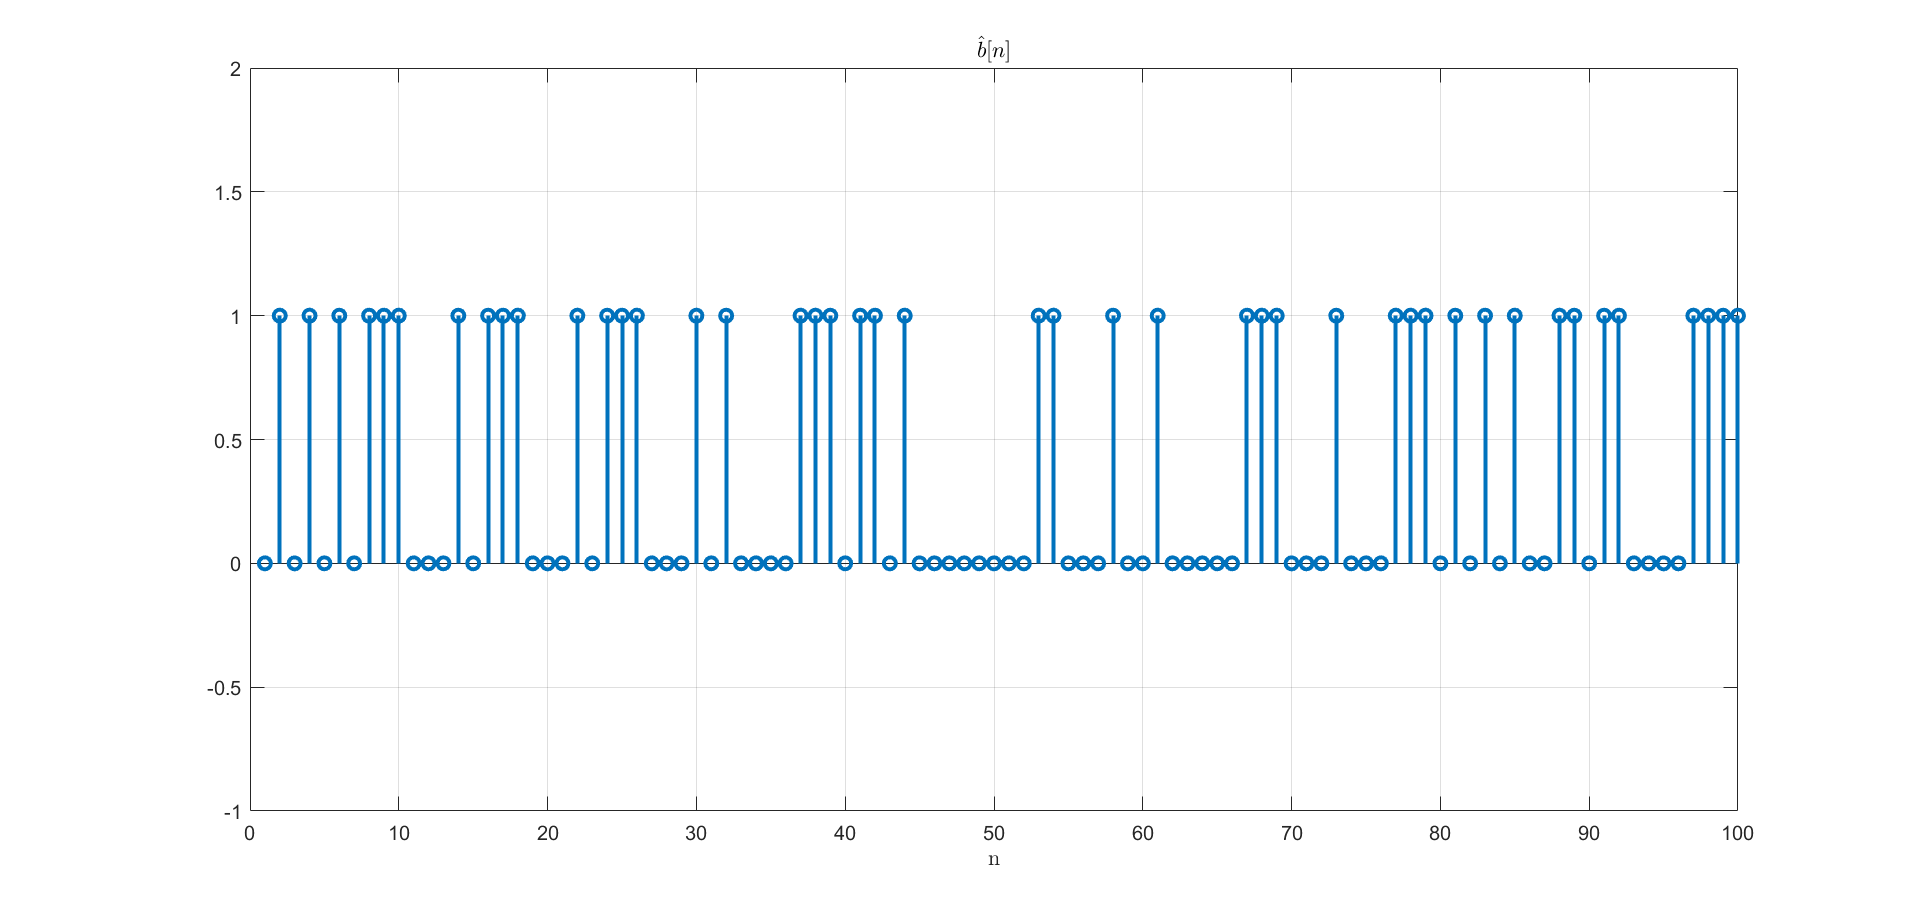
\includegraphics[width=0.8\textwidth]{comsys_fig47.png}\\ 
		\centering
	\end{figure}
	\begin{figure}[H]
		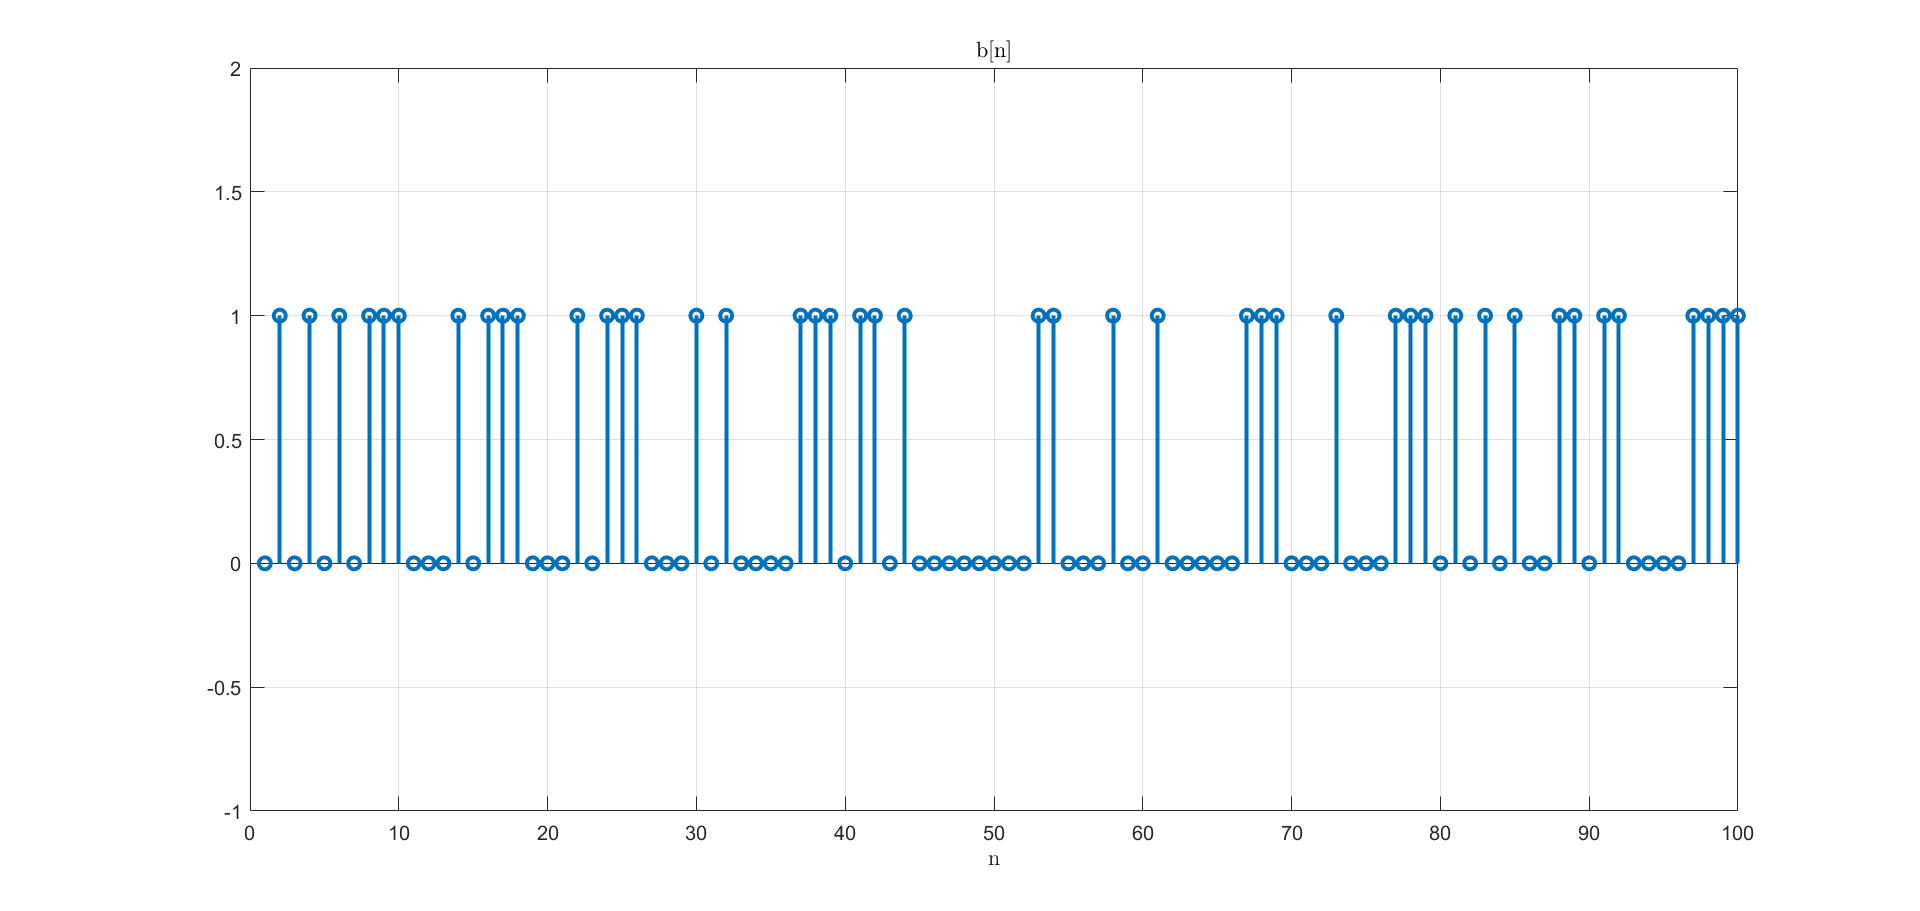
\includegraphics[width=0.8\textwidth]{comsys_fig48.png}\\ 
		\centering
	\end{figure}
	می توان دید که در این مدولاسیون هم در حالت بدون نویز سیگنال بدون خطا منتقل می شود.
	\subsubsection*{ج}
	\begin{figure}[H]
		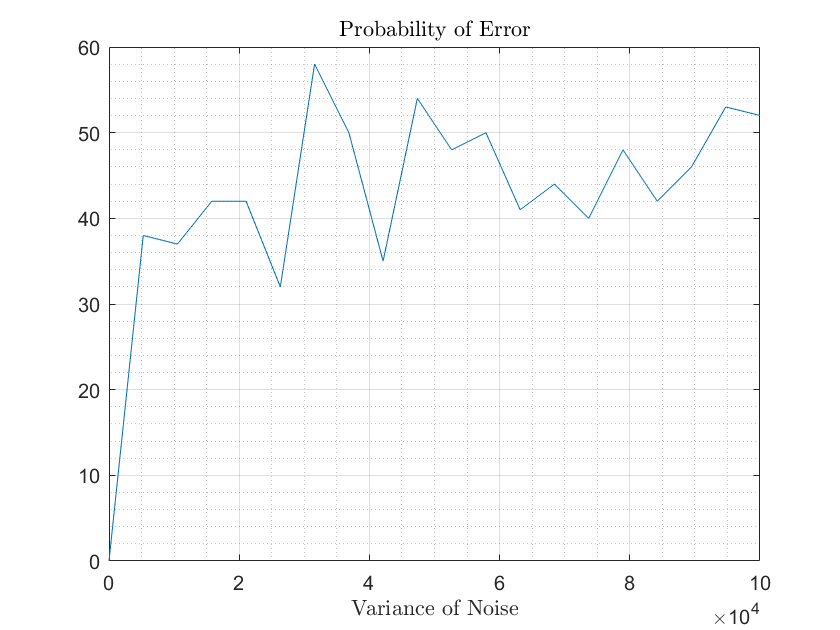
\includegraphics[width=0.8\textwidth]{comsys_fig49.png}\\ 
		\centering
	\end{figure}
	می بینیم که در مدولاسیون \lr{FSK} خطا حتی تا حدود 60 درصد هم می رسد و از دو مدولاسیون قبلی بیشتر است.
	\subsubsection*{د}
	می توان مشاهده کرد که در این مدولاسیون نسبت به مدولاسیون های قبلی خطا بیشتر است و به ازای واریانس های کمتر نسبت به حالت های قبل پراکندگی و خطای نسبتا زیادی داریم.
	\begin{figure}[H]
		\includegraphics[width=0.8\textwidth]{comsys_fig50.png}\\ 
		\centering
	\end{figure}
	\subsection{}
	مدولاسیون \lr{FSK} نسبت به دو مدولاسیون دیگر به پهنای باند بیشتری نیاز دارد.برای حالت معرفی شده در این پروژه برای مدولاسیون \lr{FSK} نیاز به حداقل 3 کیلوهرتز پهنای باند داریم درحالی که پهنای باند کانال برابر 1 کیلوهرتز است و برای استفاده از مدولاسیون \lr{FSK} چندان مناسب نیست.
	\newline
	همچنین دیدیم که در مدولاسیون \lr{FSK} خطا بیشتر است و به بیان دیگر حساسیت بیشتری به نویز نسبت به دو مدولاسیون دیگر داریم.
	\section{انتقال دنباله ای از اعداد  ۸بیتی}
	\subsection{}
	تابع های مورد نظر با کمک تابع های \lr{de2bi} و \lr{bi2de} متلب پیاده سازی شدند.
	\subsection{}
	مشاهده می شود که با افزایش واریانس خطا افزایش پیدا می کند.
	\begin{figure}[H]
		\includegraphics[width=0.8\textwidth]{comsys_fig51.png}\\ 
		\centering
	\end{figure}
	\subsection{}
	به ازای چند مقدار مختلف واریانس توزیع خطا را رسم می کنیم.
		\begin{figure}[H]
		\includegraphics[width=0.8\textwidth]{comsys_fig52.png}\\ 
		\centering
	\end{figure}
		\begin{figure}[H]
		\includegraphics[width=0.8\textwidth]{comsys_fig53.png}\\ 
		\centering
	\end{figure}
		\begin{figure}[H]
		\includegraphics[width=0.8\textwidth]{comsys_fig54.png}\\ 
		\centering
	\end{figure}
		\begin{figure}[H]
		\includegraphics[width=0.8\textwidth]{comsys_fig55.png}\\ 
		\centering
	\end{figure}
		\begin{figure}[H]
		\includegraphics[width=0.8\textwidth]{comsys_fig56.png}\\ 
		\centering
	\end{figure}
		\begin{figure}[H]
		\includegraphics[width=0.8\textwidth]{comsys_fig57.png}\\ 
		\centering
	\end{figure}
	\section{فِشُرگُستَر!}
	\subsection{}
	\begin{figure}[H]
		\includegraphics[width=0.8\textwidth]{comsys_fig58.png}\\ 
		\centering
	\end{figure}
	مشاهده می شود که به به ازای 
	$\mu$
	های کوچک نمودار تقریبا خطی است و با افزایش 
	$\mu$
	نمودار غیرخطی تر می شود.
	\subsection{}
	در این قسمت از حکایت شماره 14 از باب هفتم گلستان سعدی با صدای زیبای خسرو شکیبایی استفاده شده است و از سیگنال نمونه برداری شده است.
	\subsection{}
	توان سیگنال بعد از بهنجار شدن برابر  با 
	$-15.8426
	db$
	است.
	\subsection{}
	تابع پیاده سازی شده به این صورت است:
\begin{latin*}
	\begin{lstlisting}[language=Matlab]
		function output = ulaw_compressor(x , mu)
		output = sign(x) .* (log(1 + mu.*abs(x)) / log(1 + mu));
		end
	\end{lstlisting}
\end{latin*}
\subsection{}
تابع پیاده سازی شده در این بخش سیگنال اصلی را از سیگنال فشرده شده استخراج می کند.
\begin{latin*}
	\begin{lstlisting}[language=Matlab]
		function x =   ulaw_expander(y , mu)
		x =  sign(y) .* (1/mu) .* ((1 + mu) .^ abs(y) - 1);
		end
	\end{lstlisting}
\end{latin*}
\subsection{}
سیگنال ورودی به این شکل است:
\begin{figure}[H]
	\includegraphics[width=0.8\textwidth]{comsys_fig59.png}\\ 
	\centering
\end{figure}
\newpage
به ازای چند مقدار 
$\mu$
سیگنال بازسازی شده را رسم می کنیم و مقدار خطای \lr{RMS} را به دست می آوریم.
\begin{itemize}
	\item 
	$\mu = 1$
	\begin{figure}[H]
		\includegraphics[width=0.7\textwidth]{comsys_fig60.png}\\ 
		\centering
	\end{figure}
	\begin{flushleft}
		$RMS error = 6.6058e-17$
	\end{flushleft}
	
		\item 
	$\mu = 30$
	\begin{figure}[H]
		\includegraphics[width=0.7\textwidth]{comsys_fig61.png}\\ 
		\centering
	\end{figure}
	\begin{flushleft}
		$RMS error = 3.1926e-17$
	\end{flushleft}
	
	\item 
	$\mu = 80$
	\begin{figure}[H]
		\includegraphics[width=0.7\textwidth]{comsys_fig62.png}\\ 
		\centering
	\end{figure}
	\begin{flushleft}
		$RMS error = 5.5173e-17$
	\end{flushleft}
	
	\item 
	$\mu = 150$
	\begin{figure}[H]
		\includegraphics[width=0.7\textwidth]{comsys_fig63.png}\\ 
		\centering
	\end{figure}
	\begin{flushleft}
		$RMS error = 4.8456e-17$
	\end{flushleft}
	
	\item 
	$\mu = 255$
	\begin{figure}[H]
		\includegraphics[width=0.7\textwidth]{comsys_fig64.png}\\ 
		\centering
	\end{figure}
	\begin{flushleft}
		$RMS error = 5.4743e-17$
	\end{flushleft}
	
	
\end{itemize}
\subsection{}
تابع پیاده شده به این صورت است:
\begin{latin*}
	\begin{lstlisting}[language=Matlab]
		function quantized_signal = quantizer(signal, L)
		max_val = max(signal);
		min_val = min(signal);
		delta = (max_val - min_val) / L;
		quantized_signal = round(signal / delta) * delta;
		end
	\end{lstlisting}
\end{latin*}
\subsection{}
سیگنال کوانتیزه شده و مقدار \lr{SNR} برای مقادیر مختلف \lr{L} در ادامه آورده شده است.
\begin{itemize}
	\item 
	\lr{L = 4}
	\begin{figure}[H]
		\includegraphics[width=0.7\textwidth]{comsys_fig65.png}\\ 
		\centering
	\end{figure}
	\begin{flushleft}
		$SNR = 3.0005$\\
		$SNR_{db} = 4.7719$
	\end{flushleft}
	\item 
	\lr{L = 5}
	\begin{figure}[H]
		\includegraphics[width=0.7\textwidth]{comsys_fig66.png}\\ 
		\centering
	\end{figure}
	\begin{flushleft}
		$SNR = 4.0843$\\
		$SNR_{db} = 6.1111$
	\end{flushleft}
	\item 
	\lr{L = 6}
	\begin{figure}[H]
		\includegraphics[width=0.7\textwidth]{comsys_fig67.png}\\ 
		\centering
	\end{figure}
	\begin{flushleft}
		$SNR = 5.2863$\\
		$SNR_{db} = 7.2315$
	\end{flushleft}
	\item 
	\lr{L = 7}
	\begin{figure}[H]
		\includegraphics[width=0.7\textwidth]{comsys_fig68.png}\\ 
		\centering
	\end{figure}
	\begin{flushleft}
		$SNR = 6.6556$\\
		$SNR_{db} = 8.2319$
	\end{flushleft}
	\item 
	\lr{L = 8}
	\begin{figure}[H]
		\includegraphics[width=0.7\textwidth]{comsys_fig69.png}\\ 
		\centering
	\end{figure}
	\begin{flushleft}
		$SNR = 8.1239$\\
		$SNR_{db} = 9.0976$
	\end{flushleft}
\end{itemize}
می بینیم که با افزایش سطوح مقدار \lr{SNR} افزایش پیدا می کند که برای ما مطلوب تر است.
\subsection{}
\subsubsection{\lr{L = 4}}
\begin{itemize}
	\item 
	$\mu = 1$
	\begin{flushleft}
		$SNR = 3.5905$\\
		$SNR_{db} = 5.5516$
	\end{flushleft}
	\item 
	$\mu = 5$
	\begin{flushleft}
		$SNR = 3.9337$\\
		$SNR_{db} = 5.9480$
	\end{flushleft}
	\item 
	$\mu = 30$
	\begin{flushleft}
		$SNR = 2.1398$\\
		$SNR_{db} = 3.3037$
	\end{flushleft}
	\item 
	$\mu = 80$
	\begin{flushleft}
		$SNR = 1.2403$\\
		$SNR_{db} = 0.9354$
	\end{flushleft}
	\item 
	$\mu = 150$
	\begin{flushleft}
		$SNR = 0.8718$\\
		$SNR_{db} = -0.5956 $
	\end{flushleft}
	\item 
	$\mu = 255$
	\begin{flushleft}
		$SNR = 0.6579$\\
		$SNR_{db} = -1.8181 $
	\end{flushleft}
\end{itemize}

\subsubsection{\lr{L = 5}}
\begin{itemize}
	\item 
	$\mu = 1$
	\begin{flushleft}
		$SNR = 5.1848$\\
		$SNR_{db} = 7.1474$
	\end{flushleft}
	\item 
	$\mu = 5$
	\begin{flushleft}
		$SNR = 6.3970$\\
		$SNR_{db} = 8.0598$
	\end{flushleft}
	\item 
	$\mu = 30$
	\begin{flushleft}
		$SNR = 5.0393$\\
		$SNR_{db} = 7.0237$
	\end{flushleft}
	\item 
	$\mu = 80$
	\begin{flushleft}
		$SNR = 3.9879$\\
		$SNR_{db} = 6.0074$
	\end{flushleft}
	\item 
	$\mu = 150$
	\begin{flushleft}
		$SNR = 3.4606$\\
		$SNR_{db} = 5.3915 $
	\end{flushleft}
	\item 
	$\mu = 255$
	\begin{flushleft}
		$SNR = 3.0947$\\
		$SNR_{db} = 4.9062 $
	\end{flushleft}
\end{itemize}

\subsubsection{\lr{L = 6}}
\begin{itemize}
	\item 
	$\mu = 1$
	\begin{flushleft}
		$SNR = 6.9027$\\
		$SNR_{db} = 8.3902$
	\end{flushleft}
	\item 
	$\mu = 5$
	\begin{flushleft}
		$SNR = 8.6262$\\
		$SNR_{db} = 9.3582$
	\end{flushleft}
	\item 
	$\mu = 30$
	\begin{flushleft}
		$SNR = 6.0284$\\
		$SNR_{db} = 7.8020$
	\end{flushleft}
	\item 
	$\mu = 80$
	\begin{flushleft}
		$SNR = 3.8335 $\\
		$SNR_{db} = 5.8359$
	\end{flushleft}
	\item 
	$\mu = 150$
	\begin{flushleft}
		$SNR = 2.8065$\\
		$SNR_{db} = 4.4816 $
	\end{flushleft}
	\item 
	$\mu = 255$
	\begin{flushleft}
		$SNR = 2.1732$\\
		$SNR_{db} = 3.3710$
	\end{flushleft}
\end{itemize}

\subsubsection{\lr{L = 7}}
\begin{itemize}
	\item 
	$\mu = 1$
	\begin{flushleft}
		$SNR = 8.9386$\\
		$SNR_{db} = 9.5127$
	\end{flushleft}
	\item 
	$\mu = 5$
	\begin{flushleft}
		$SNR = 11.8991$\\
		$SNR_{db} = 10.7551$
	\end{flushleft}
	\item 
	$\mu = 30$
	\begin{flushleft}
		$SNR = 9.8743$\\
		$SNR_{db} = 9.9450$
	\end{flushleft}
	\item 
	$\mu = 80$
	\begin{flushleft}
		$SNR = 7.2001$\\
		$SNR_{db} = 8.5734$
	\end{flushleft}
	\item 
	$\mu = 150$
	\begin{flushleft}
		$SNR = 5.8732 $\\
		$SNR_{db} = 7.6888 $
	\end{flushleft}
	\item 
	$\mu = 255$
	\begin{flushleft}
		$SNR = 5.0471$\\
		$SNR_{db} = 7.0304$
	\end{flushleft}
\end{itemize}

\subsubsection{\lr{L = 8}}
\begin{itemize}
	\item 
	$\mu = 1$
	\begin{flushleft}
		$SNR = 11.0240$\\
		$SNR_{db} = 10.4234$
	\end{flushleft}
	\item 
	$\mu = 5$
	\begin{flushleft}
		$SNR = 14.9818$\\
		$SNR_{db} = 11.7556$
	\end{flushleft}
	\item 
	$\mu = 30$
	\begin{flushleft}
		$SNR = 11.5073$\\
		$SNR_{db} = 10.6098$
	\end{flushleft}
	\item 
	$\mu = 80$
	\begin{flushleft}
		$SNR = 7.7416 $\\
		$SNR_{db} = 8.8883$
	\end{flushleft}
	\item 
	$\mu = 150$
	\begin{flushleft}
		$SNR = 5.9050$\\
		$SNR_{db} = 7.7122 $
	\end{flushleft}
	\item 
	$\mu = 255$
	\begin{flushleft}
		$SNR = 4.6961$\\
		$SNR_{db} = 6.7174$
	\end{flushleft}
\end{itemize}
می توان دید که افزایش 
$\mu$
ابتدا باعث افزایش و سپس باعث کاهش \lr{SNR} می شود؛ درحالی که افزایش \lr{L} باعث افزایش \lr{SNR} می شود.
\subsection{}
\begin{figure}[H]
	\includegraphics[width=0.7\textwidth]{comsys_fig70.png}\\ 
	\centering
\end{figure}
\subsection{}
به عنوان مثال حالت \lr{L= 6} را بررسی می کنیم.
\begin{itemize}
	\item 
	$\mu = 1$
	\begin{flushleft}
		$SNR = 3.9498$\\
		$SNR_{db} = 5.9657$
	\end{flushleft}
	\item 
	$\mu = 5$
	\begin{flushleft}
		$SNR = 2.5306$\\
		$SNR_{db} = 4.0322$
	\end{flushleft}
	\item 
	$\mu = 30$
	\begin{flushleft}
		$SNR = 1.6017$\\
		$SNR_{db} = 2.0457$
	\end{flushleft}
	\item 
	$\mu = 80$
	\begin{flushleft}
		$SNR = 1.3898 $\\
		$SNR_{db} = 1.4297$
	\end{flushleft}
	\item 
	$\mu = 150$
	\begin{flushleft}
		$SNR = 1.3115$\\
		$SNR_{db} = 1.1778$
	\end{flushleft}
	\item 
	$\mu = 255$
	\begin{flushleft}
		$SNR = 1.2624$\\
		$SNR_{db} = 1.0118$
	\end{flushleft}
\end{itemize}
می توان مشاهده کرد که مقدار \lr{SNR} نسبت به حالت قبل کاهش پیدا کرده است.این یعنی نسبت توان سیگنال به توان نویز کاهش پیدا کرده است که مطلوب نیست بنابراین بهتر است از همان ترتیب قبل استفاده کنیم.

\end{document}
